\documentclass[11pt]{article}
%
%--------------------   start of the 'preamble'
%
\usepackage{fullpage}
\usepackage[latin1]{inputenc}
\usepackage[T1]{fontenc}
\usepackage{lmodern}
\usepackage{amsmath}
\usepackage{amsfonts}
\usepackage{amssymb}
\usepackage[bookmarks=true,bookmarksnumbered=true,colorlinks=false,pdfborder={0 0 0}]{hyperref}
\usepackage{picinpar, wrapfig}
\usepackage{array, multirow, hhline, tabularx, graphicx}

\usepackage{cite}

\numberwithin{equation}{section}
\numberwithin{figure}{section}
\numberwithin{table}{section}

\title{State estimation for polyhedral hybrid systems and applications to the Cell Transmission Model - DRAFT}
\date{\today}
\author{
        %\large
        \textsc{Jerome Thai}
        \thanks{Corresponding Author, Department of Electrical Engineering and Computer Science, University of California, Berkeley, jerome.thai@berkeley.edu}
}

\begin{document}

\maketitle

\begin{abstract}

abstract

\end{abstract}

\section{Introduction}

Numerous traffic estimation techniques developed in the literature rely on density based traffic models such as the Lighthill-Whitham-Richards (LWR) partial differential equation (PDE) \cite{Lighthill1955,Richards1956} and its discretization using the Godunov scheme \cite{Lebacque1996,LeVeque1992,Strub2006} (also known as the Cell Transmission Model (CTM) \cite{Daganzo1994,Daganzo1995} in the transportation literature). These highway traffic monitoring systems rely on large amounts of data from different sources. These include \textit{inductive loop detectors} (ILD) used in the PeMS system \cite{Chen2005} and \textit{in-vehicle transponders} (IVTs) such as FasTrak. Recently, the available data on traffic has increased tremendously since the development of cellular phone based highway traffic monitoring. With the cellular phone communication infrastructure in place and privacy aware smartphone sensing technology in full expansion \cite{Hoh2008}, a large volume of data from mobile devices is now available \cite{Herrera2009}. Large scale Applications include traffic flow estimation to assimilate velocity measurements \cite{Work2008,Work2008a}, which is a rapidly expanding field at the heart of mobile internet services. This points out on the necessity of powerful statistical filters and algorithms to efficiently assimilate the measurements.

In \cite{Work2008,Work2008a} the \textit{Ensemble Kalman Filter} is used to assimilate velocity measurements. In \cite{Munoz2003}, a switching-mode model (SMM) has been derived from the CTM, which is a nonlinear discrete time dynamical system. This consists in switching among different sets of linear difference equations, defined as linear state-space model (SSM) or modes, combined with a hidden Markov model to describe the transitions from one mode to another. The Mixture Kalman filter algorithm \cite{Chen2000} is employed to assimilate data in a switching state-space model. In this paper, we show that for a Daganzo-Newell fundamental diagram, the Godunov scheme applied to the LWR model (described in \cite{Daganzo1995}) is a piecewise affine (PWA) dynamic system, where each affine component is a linear mode. Contrary to the SMM, where an additional statistical model, namely the hidden Markov model, is introduced, we unravel the PWA character of the original CTM.


\section{Traffic flow modelling}

\subsection{The LWR Model}

Lighthill and Whitham in 1955 \cite{Lighthill1955} introduce a macroscopic dynamic model of traffic based on conservation of cars (\ref{eq:LWRmodel1}), using Greenshields' hypothesis \cite{Greenshields1934} of a static flow/density relationship (\ref{eq:LWRmodel2}), known as the \textit{fundamental diagram}. The model consists of the following two equations:

\begin{equation} \label{eq:LWRmodel1}
\frac{\partial \rho(x,t)}{\partial t} + \frac{\partial q(x,t)}{\partial x} = 0
\end{equation}

\begin{equation} \label{eq:LWRmodel2}
q(x,t) = Q(\rho(x,t))
\end{equation}

\noindent where $\rho(x,t)$ and $q(x,t)$ denote the density and the flow of vehicles at location x and time t respectively, and $Q$ is the flux function which is assumed to be a function of the density only. 

Equation (\ref{eq:LWRmodel1}) is the principle of conservation of mass, or in this case conservation of vehicles, from fluid dynamics. These equations can be written more compactly as:

\begin{equation} \label{eq:LWRmodel3}
\frac{\partial \rho(x,t)}{\partial t} + Q'(\rho(x,t))\frac{\partial \rho(x,t)}{\partial x} = 0
\end{equation}

This equation is commonly known as the \textit{Lighthill-Whitham-Richards}, or LWR, model. Different fundamental diagrams have been suggested. Greenshields \cite{Greenshields1934} found that freeway speed and density could be reasonably well approximated by a straight line. The expression of the velocity and the flux are then:

\begin{equation} \label{eq:greenshieldsVelocity}
v = V_{G}(\rho) = v_{f}(1-\frac{\rho}{\rho_{\text{jam}}})
\end{equation}

\begin{equation} \label{eq:greenshieldsFlux}
Q_{G}(\rho) = \rho V_{G}(\rho) = v_{f}(\rho-\frac{\rho^{2}}{\rho_{\text{jam}}})
\end{equation}

where $v_{f}$ is the free flow (or maximum) velocity, and $\rho_{\text{jam}}$ is the jam (or maximum) density. In this case, the flow is a quadratic function of the density. 

Many researchers have later suggested alternative shapes that provide a better fit to the measured data. They all share the same characteristics \textbf{LWR1-6}:

LWR1. Greenshields' hypothesis of a static flow/density relationship: $q = Q(\rho(x,t))$

LWR2. $Q(0)=Q(\rho_{\text{jam}})$=0

LWR3. The continuous portions of $Q(\rho)$ are concave.

LWR4. $V(0) = v_{f}$, and $V(\rho_{\text{jam}}) = 0$.

LWR5. A critical density $\rho_{c}$ can be defined where the maximum flow $q_{c}$ is attained. Then, $Q(\rho)$ is increasing for $\rho \leq \rho_{c}$ and decrasing for $\rho > \rho_{c}$.

LWR6. The critical density $\rho_{c}$ separates the fundamental diagram into two regimes: \textit{free flow} when $\rho \leq \rho_{c}$ and \textit{congestion} when $\rho > \rho_{c}$

\begin{figure}[ht]
  \centering
    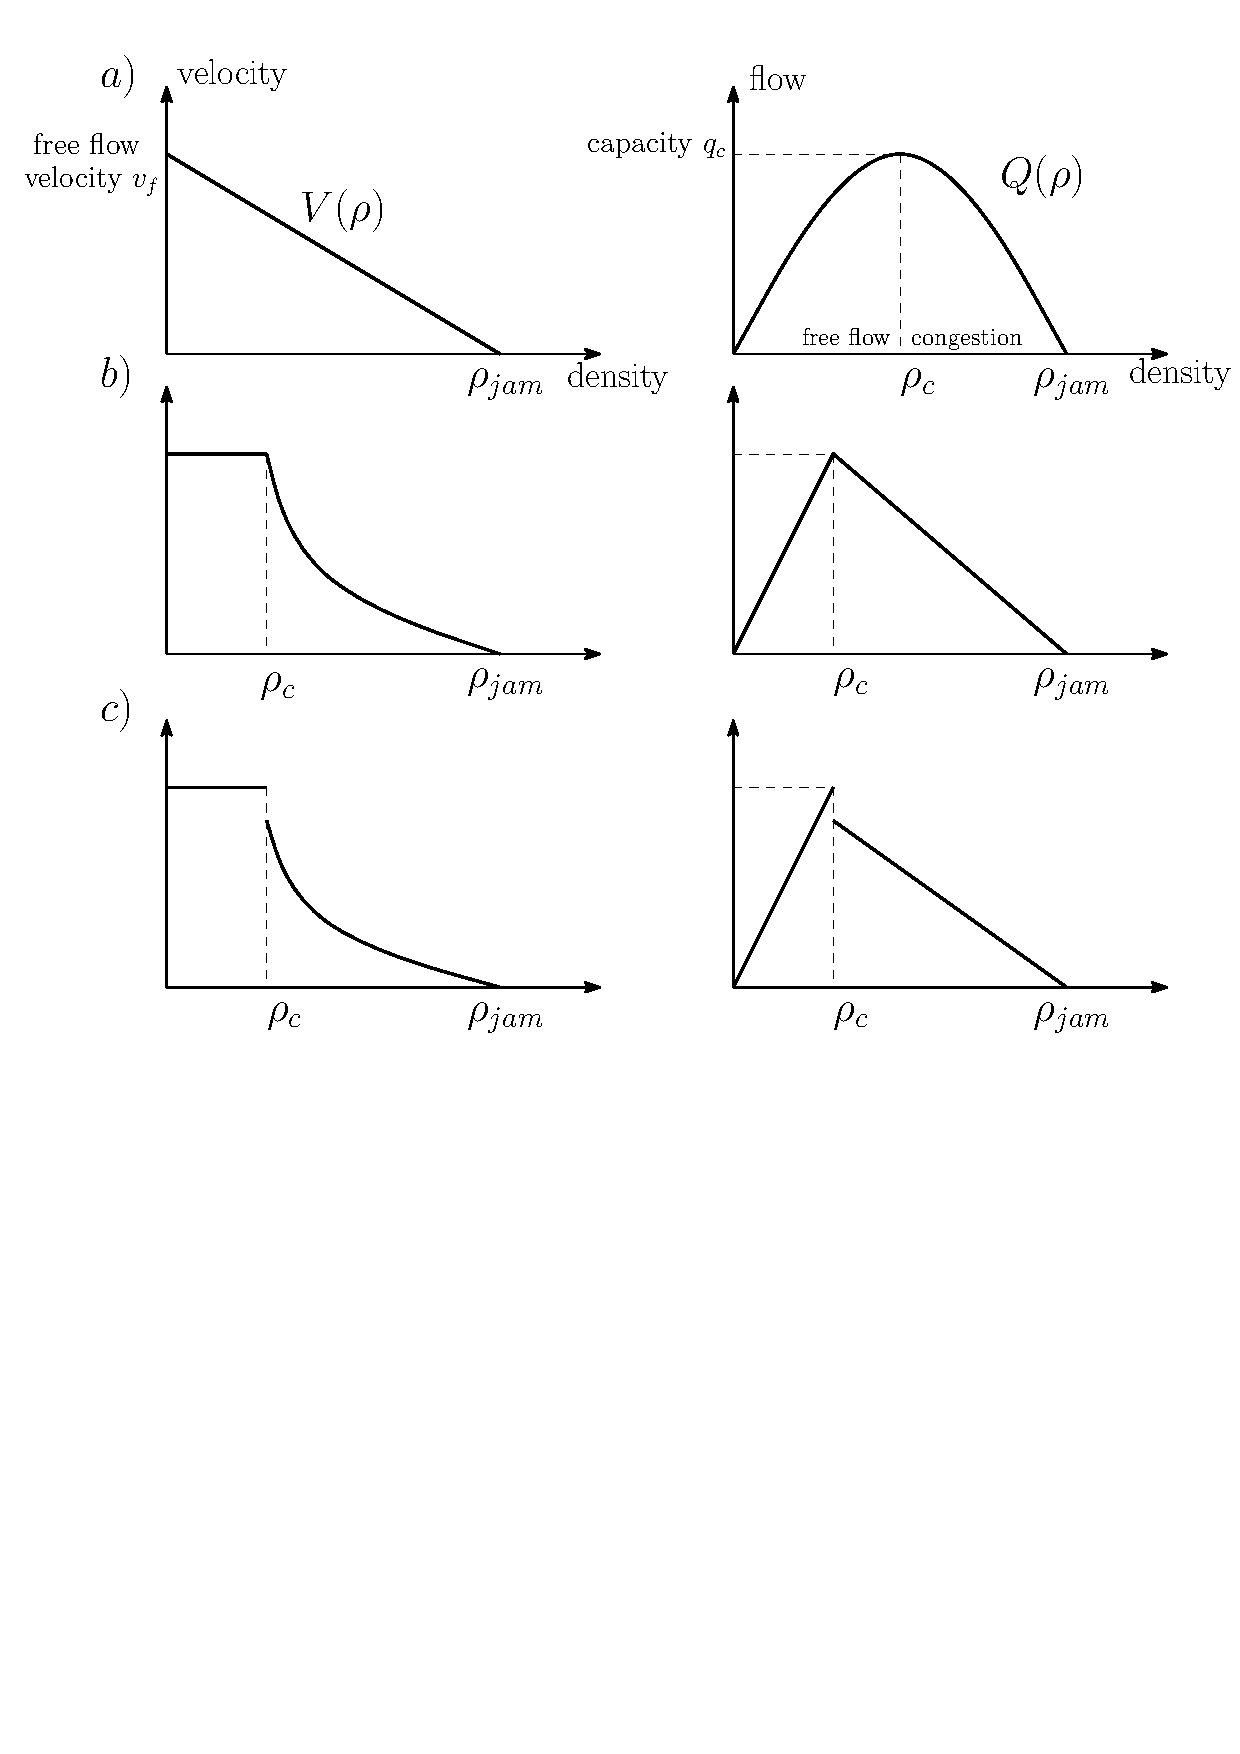
\includegraphics[width=12cm]{fundamentalDiagram2.pdf}
    \caption{Speed and flow relationships (fundamental diagrams) for Greenshields (a), Daganzo-Newell (b), and discontinuous (c).}
    \label{fig:fundamentalDiagram}
\end{figure}

Many researchers have later suggested alternative shapes that provide a better fit to the measured data. For instance, the widely used Daganzo-Newell velocity function assumes a constant velocity in free-flow and a hyperbolic velocity in congestion as shown in Figure \ref{fig:fundamentalDiagram}:
\noindent 
\begin{equation}\label{eq:dnVelocity}
v = V_{DN}(\rho) = \begin{cases}
v_{f} & \text{if } \rho \leq \rho_{c} \\
-\omega_{f} \left( 1 - \frac{\rho_{\text{jam}}}{\rho} \right) & \text{if } \rho > \rho_{c}
\end{cases}
\end{equation}

\noindent and the corresponding flux function is:

\begin{equation}\label{eq:dnFlux}
Q_{DN}(\rho) = \rho V_{DN}(\rho) = \begin{cases}
v_{f} \rho & \text{if } \rho \leq \rho_{c} \\
-\omega_{f} \left( \rho - \rho_{\text{jam}} \right) & \text{if } \rho > \rho_{c}
\end{cases}
\end{equation}

\noindent where $\omega_{f}=v_{f}\rho_{c}/(\rho_{\text{jam}}-\rho_{c})$ is the backwards propagation wave speed.

Measurements on the free-flow side are usually well represented by a straight line, whereas measurements in congestion tend to be more scattered. Some authors claim that there is a difference in the maximum measured flow $Q(\rho_{c})$, depending on whether the freeway is in free-flow or congestion, and contend that a \textit{discontinuity} exists at $\rho=\rho_{c}$ as in Figure \ref{fig:fundamentalDiagram}. This is described in \cite{Agyemang-Duah1991,Cassidy1999,Hall1991} as a \textit{capacity drop}, on the order of 4-10\% in peak flow, as the freeway transitions into congestion.

\subsection{Numerical Discretization}

A good numerical method to solve the equations along roads is represented by the Godunov scheme, which is based on exact solutions to Riemann problems \cite{Godlewski1996,Godunov1959}. This leads to the construction of a nonlinear discrete time dynamical system.

The Godunov discretization scheme is applied on the LWR PDE, where the discrete time step $\Delta t$ is indexed by $t$, and the discrete space step $\Delta x$ is indexed by $i$:

\begin{equation} \label{eq:rhoGodunov}
\rho^{t+1}_{i} = \rho^{t}_{i} - \frac{\Delta t}{\Delta x}\left(G(\rho^{t}_{i},\rho^{t}_{i+1})-G(\rho^{t}_{i-1},\rho^{t}_{i})\right)
\end{equation}

\noindent In order to ensure numerical stability, the time and space steps are coupled by the CFL condition \cite{LeVeque1992}: $c_{max}\frac{\Delta t}{\Delta x} \leq 1$ where $c_{max}$ denotes the maximal characteristic speed.

For a family of flux functions $Q(\rho)$ that share the same characteristics \textbf{LWR1-6} listed above, the Godunov flux can be expressed as the minimum of the \textit{sending flow} from the upstream cell and the \textit{receiving flow} from the downstream cell through a boundary connecting two cells of a homogeneous road (i.e. the upstream and downstream cells have the same characteristics) \footnotemark. The \textit{sending flow} $S(\rho)$ is equal to the upstream flow if the upstream traffic is in free flow ($\rho \leq \rho_{c}$) or the capacity of the upstream section $q_{c}$ if the upstream traffic is in congestion ($\rho > \rho_{c}$); on the other hand, the \textit{receiving flow} $R(\rho)$ is equal to the capacity of the downstream section if the downstream traffic is in free flow or the downstream flow if the downstream traffic is in congestion. For this model, we note that for an heterogeneous segment (for instance due to a change in the number of lanes) a fundamental diagram with different parameters is defined at each cell $i$, consequently we add a subscript: $Q_{i}(\rho)$, $S_{i}(\rho)$, $R_{i}(\rho)$ and there is an implicit subscript for $G(\rho_{i},\rho_{i+1})$.

\footnotetext{
There are various definitions of the Godunov flux $G(\rho_{1},\rho_{2})$ in the literature, notably in \cite{Garavello2006}:

\begin{equation} \label{eq:rhoGodunovFluxGeneral}
G(\rho_{1},\rho_{2}) = \begin{cases}
\text{min}_{\rho \in [\rho_{1},\rho_{2}]} Q(\rho) & \text{if } \rho_{1} \leq \rho_{2}\\
\text{max}_{\rho \in [\rho_{2},\rho_{1}]} Q(\rho) & \text{if } \rho_{2} \leq \rho_{1}
\end{cases}
\end{equation}
\noindent This assumes that a fundamental diagram is defined at each boundary between two cells, which differs from the CTM.
}

\begin{equation} \label{eq:rhoGodunovFlux1}
G(\rho_{1},\rho_{2}) = \text{min}(S_{1}(\rho_{1}),R_{2}(\rho_{2}))
\end{equation}

\begin{equation} \label{eq:sendingFlow1}
S_{1}(\rho) = \begin{cases}
Q_{1}(\rho) & \text{if } \rho \leq \rho_{c1} \\
q_{c1} &  \text{if } \rho > \rho_{c1}
\end{cases}
\end{equation}

\begin{equation} \label{eq:receivingFlow1}
R_{2}(\rho) = \begin{cases}
q_{c2} & \text{if } \rho \leq \rho_{c2} \\
Q_{2}(\rho) &  \text{if } \rho > \rho_{c2}
\end{cases}
\end{equation}

\noindent where $\rho_{1}$ is the density of the cell upstream and $\rho_{2}$ is the density of the cell downstream. Then sending and receiving flows for the Daganzo-Newell fundamental diagram is:

\begin{equation} \label{eq:sendingFlow2}
S_{1}(\rho) = \begin{cases}
v_{f1}\rho & \text{if } \rho \leq \rho_{c1} \\
q_{c1} &  \text{if } \rho > \rho_{c1}
\end{cases}
\end{equation}

\begin{equation} \label{eq:receivingFlow2}
R_{2}(\rho) = \begin{cases}
q_{c2} & \text{if } \rho \leq \rho_{c2} \\
-\omega_{f2} \left( \rho - \rho_{\text{jam}2} \right) & \text{if } \rho > \rho_{c2}
\end{cases}
\end{equation}

\begin{figure}[ht]
  \centering
    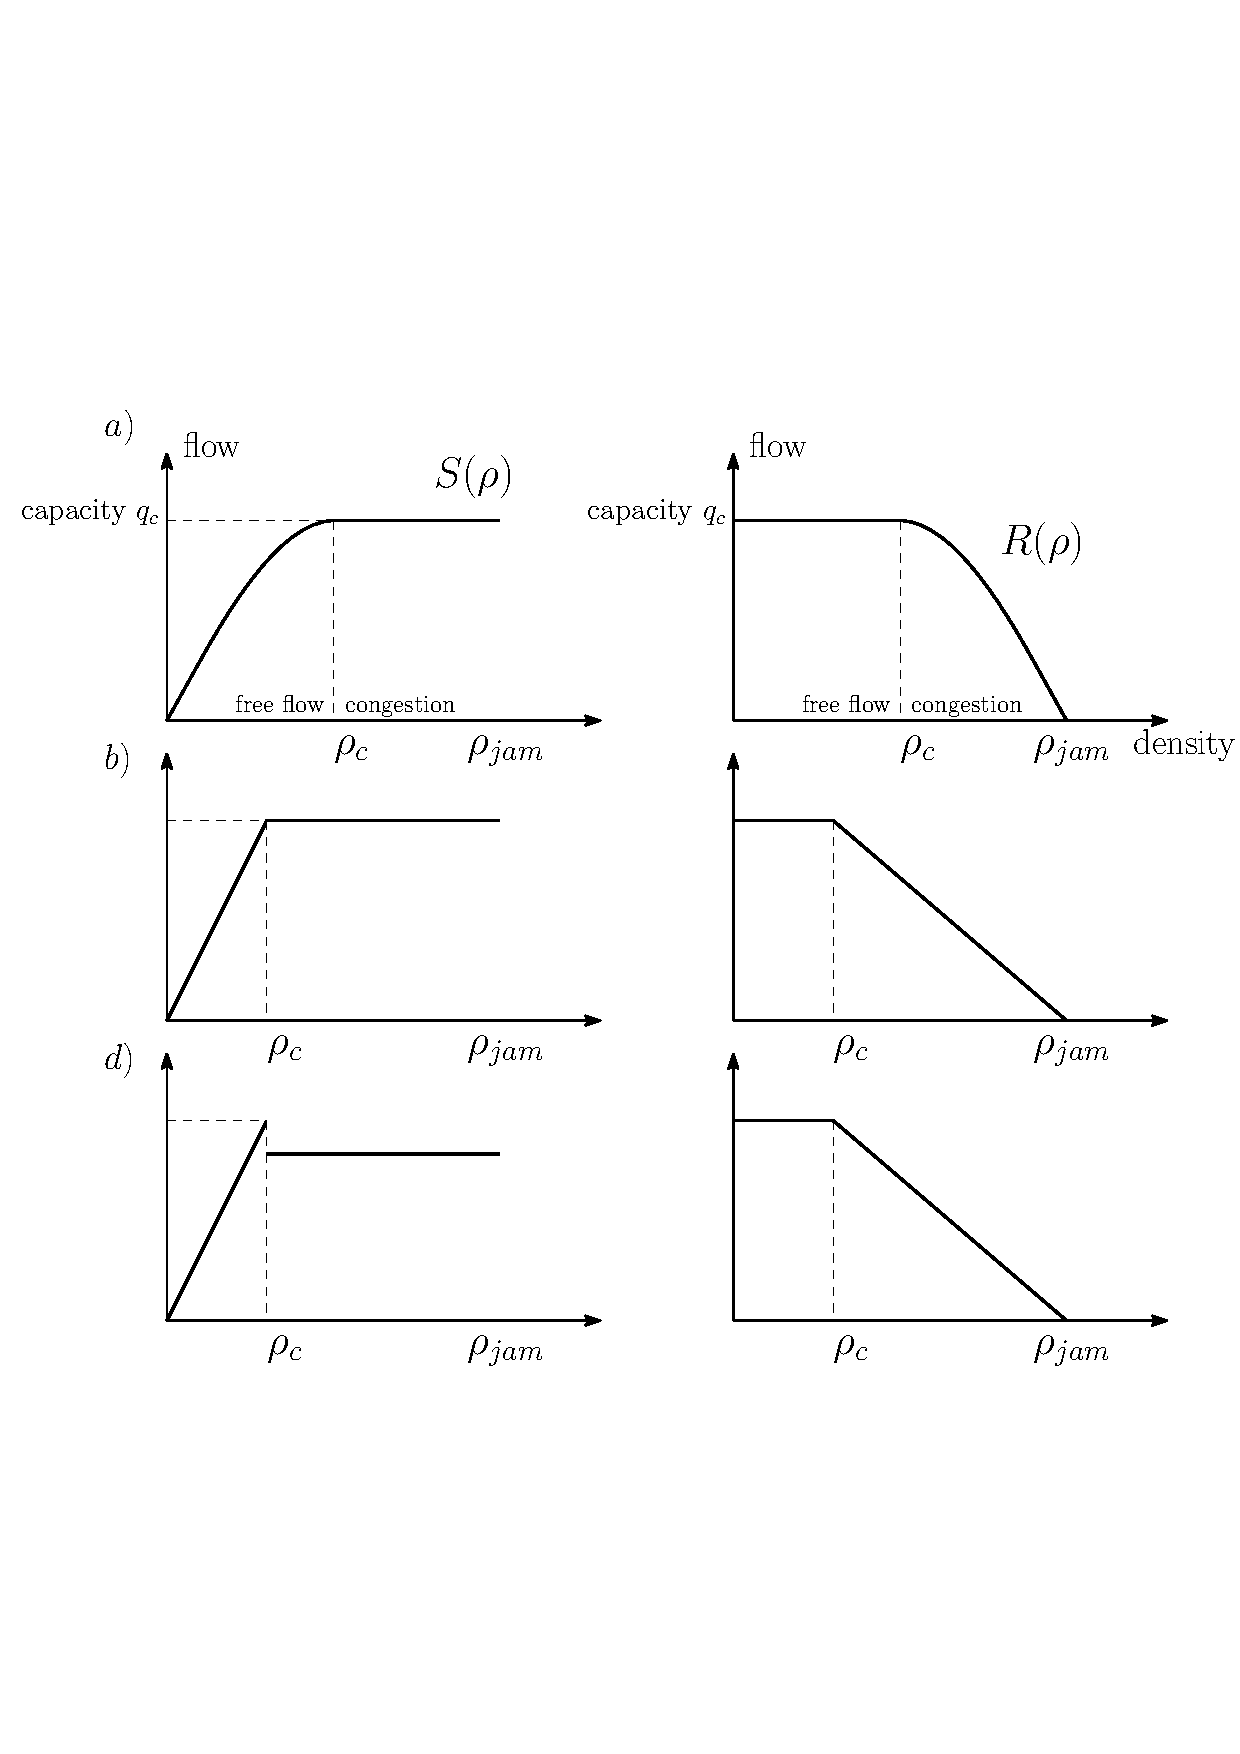
\includegraphics[width=12cm]{fundamentalDiagramSR.pdf}
    \caption{Sending and receiving flows for Greenshields (a), Daganzo-Newell (b), and discontinous (c) velocity functions.}
    \label{fig:fundamentalDiagramSR}
\end{figure}

\noindent As shown in Figure \ref{fig:fundamentalDiagramSR}, the application of the Godunov scheme to the fundamental diagrams introduces intuitive concepts of \textit{supply} and \textit{demand} at the boundary connecting two cells. The upstream cell supplies the flow at the boundary up to capicity. We can note that in the discontinuous case, there is a drop in supply capacity when the upstream traffic is in congestion, as described in \cite{Agyemang-Duah1991,Cassidy1999,Hall1991}. As a result, the flow through the boundary is smaller, even if the downstream cell can receive more flow. On the other hand, when the downstream traffic is congested, there is a decrease in demand from the downstream cell, limiting the flow through the boundary.

\hspace{10mm}

\noindent\textbf{Important remark:} For the rest of the paper, the widely-used \textit{Cell Transmission Model} (CTM) described in \cite{Daganzo1994} is chosen for our dynamic model and results are derived from it. We also suppose for simplicity and clarity that the segment of road we are modelling is homogeneous, i.e. the parameters of the fundamental diagram $\omega_{f}$, $v_{f}$, $\rho_{\text{jam}}$, $\rho_{c}$, $q_{c}$ are constant along the cells of the discretized road. And they are also time invariant because they are only related to the geometry of the highway, independently of the current traffic on it. All the results derived in the rest of the paper still remain for an heterogeneous road, in particular the piecewise affine character of the model and the tractibility of the Kalman filter algorithm, but the number of modes and the complexity increase. For more details on the heterogeneous case, see Appendix \ref{sec:CDFD}.

\hspace{10mm}

\noindent Figure \ref{fig:godunovDiagram} shows the explicit values taken by $G(\rho_{1},\rho_{2})$ for a partition of the space in different regions of the space $(\rho_{1},\rho_{2})$. We will denote by \textbf{W}, \textbf{L}, and \textbf{D} the \textit{white region}, \textit{light region}, and \textit{dark region} of the space $(\rho_{1},\rho_{2})$ respectively. 

\begin{equation}
G(\rho_{1},\rho_{2}) = \begin{cases}
R(\rho_{2}) & \text{if } (\rho_{1},\rho_{2}) \in \textbf{W}\\
q_{c} & \text{if } (\rho_{1},\rho_{2}) \in \textbf{L}\\
S(\rho_{1}) & \text{if } (\rho_{1},\rho_{2}) \in \textbf{D}
\end{cases}
\label{eq:rhoGodunovFlux}
\end{equation}

\begin{equation}
\begin{array}{ll}
\textbf{W} & = \{(\rho_{1},\rho_{2}) \mid \rho_{2} > F(\rho_{1}) \text{ ,   } \rho_{2} > \rho_{c}\}\\
\textbf{L} & = \{(\rho_{1},\rho_{2}) \mid \rho_{1} > \rho_{c} \text{ ,   } \rho_{2} \leq \rho_{c}\}\\
\textbf{D} & = \{(\rho_{1},\rho_{2}) \mid \rho_{2} \leq F(\rho_{1}) \text{ ,   } \rho_{1} \leq \rho_{c}\}
\end{array}
\label{eq:regions}
\end{equation}

\noindent where the boundary between the white and grey regions follows the $(\rho_{1},\rho_{2})=(\rho_{1},F(\rho_{1}))$ trajectory with $F(\rho_{1})= \bar{R}^{-1}(\bar{S}(\rho_{1}))$\footnotemark for $\rho_{1} \leq \rho_{c}$. $\bar{S}$ and $\bar{R}$ denote the restrictions of the sending and receiving flows to the sub-regions $[0,\rho_{c})$ and $(\rho_{c},\rho_{\text{jam}}]$ respectively, which also correspond to the left and right parts (w.r.t. $\rho_{c}$) of the fundamental diagram, as shown in the Figure \ref{fig:godunovDiagram}.

\footnotetext{Here, we formulate the more general case for equations (\ref{eq:rhoGodunovFlux}, \ref{eq:regions}) and we suppose that $\bar{R}$ is a strictly monotonic function on $(\rho_{c},\rho_{j}]$, hence invertible, and $\bar{R}^{-1}$ denotes its inverse, which is the case for the Daganzo-Newell fundamental diagram.}

\begin{figure}[ht]
  \centering
    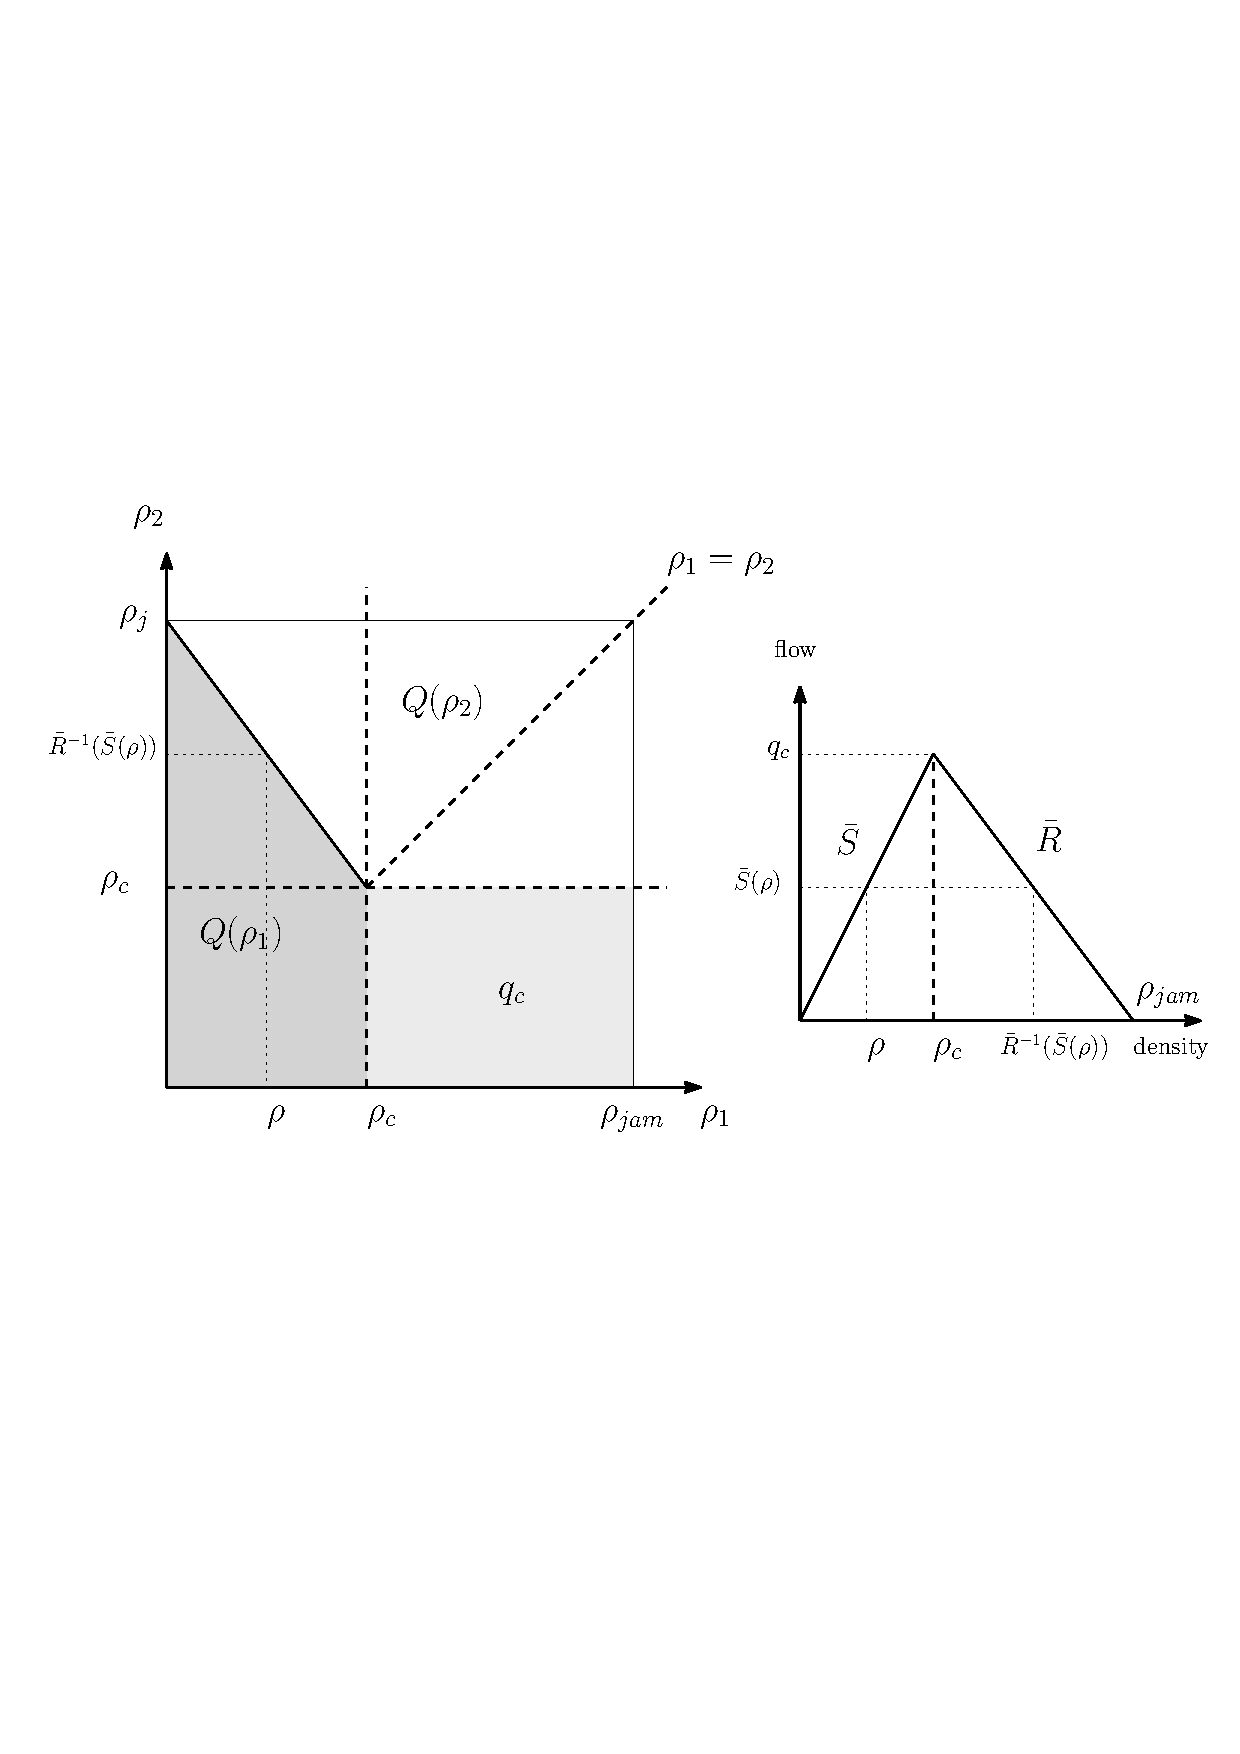
\includegraphics[width=15cm]{godunovDiagram.pdf}
    \caption{Values of $G(\rho_{1},\rho_{2})$ in the space $(\rho_{1},\rho_{2})$.}
    \label{fig:godunovDiagram}
\end{figure}

\noindent When the velocity is the Daganzo-Newell function (\ref{eq:dnVelocity}), the Godunov Flux becomes:
\begin{equation} \label{eq:rhoGodunovFlux3}
G_{DN}(\rho_{1},\rho_{2}) = \begin{cases}
-\omega_{f} \left( \rho_{2} - \rho_{\text{jam}} \right) & \text{if } (\rho_{1},\rho_{2}) \in \textbf{W}\\
q_{c} & \text{if } (\rho_{1},\rho_{2}) \in \textbf{L}\\
v_{f} \rho_{1} & \text{if } (\rho_{1},\rho_{2}) \in \textbf{D}
\end{cases}
\end{equation}

\noindent and the boundary between \textbf{W} and \textbf{D} regions is:

\begin{equation} \label{eq:boundary}
(\rho_{1},\rho_{2})=(\rho_{1},-\frac{v_{f}}{\omega_{f}}\rho_{1}+\rho_{\text{jam}})
\end{equation}

\noindent And \textbf{W}, \textbf{L}, \textbf{D} form a \textit{polyhedral partition} of the space $(\rho_{1},\rho_{2})$:

\begin{equation}
\begin{array}{ll}
\textbf{W} & = \{(\rho_{1},\rho_{2}) \mid \rho_{2} + \frac{v_{f}}{\omega_{f}}\rho_{1} > \rho_{\text{jam}} \text{ ,   } \rho_{2} > \rho_{c}\}\\
\textbf{L} & = \{(\rho_{1},\rho_{2}) \mid \rho_{1} > \rho_{c} \text{ ,   } \rho_{2} \leq \rho_{c}\}\\
\textbf{D} & = \{(\rho_{1},\rho_{2}) \mid \rho_{2} + \frac{v_{f}}{\omega_{f}}\rho_{1} \leq \rho_{\text{jam}} \text{ ,   } \rho_{1} \leq \rho_{c}\}\end{array}
\label{eq:regions2}
\end{equation}

\section{A polyhedral piecewise affine model}

In the Godunov scheme (\ref{eq:rhoGodunov}), the update of the density $\rho^{t+1}_{i}$ at cell $i$ depends on the triplet $(\rho^{t}_{i-1}, \rho^{t}_{i}, \rho^{t}_{i+1})$. In this section, we will refer to the fraction $\frac{\Delta t}{\Delta x}$ as $\alpha$. Recall the Godunov scheme reads as:

\begin{equation} \label{eq:rhoGodunov2}
\rho^{t+1}_{i} = f(\rho^{t}_{i-1},\rho^{t}_{i},\rho^{t}_{i+1}) = \rho^{t}_{i} - \alpha\left(G(\rho^{t}_{i},\rho^{t}_{i+1})-G(\rho^{t}_{i-1},\rho^{t}_{i})\right)
\end{equation}

\subsection{Decomposition in different ''modes''}\label{sec:decompositionModes}

$\rho^{t+1}_{i}$ depends on whether both pairs $(\rho^{t}_{i-1}, \rho^{t}_{i})$ and $(\rho^{t}_{i}, \rho^{t}_{i+1})$ are in \textbf{W}, \textbf{L}, or \textbf{D} via $G(\rho^{t}_{i-1},\rho^{t}_{i})$ and $G(\rho^{t}_{i},\rho^{t}_{i+1})$. So there are nine possible combinations at cell $i$, which can be reduced to seven ''modes'' since the pairs $(\rho^{t}_{i-1}, \rho^{t}_{i})$ and $(\rho^{t}_{i}, \rho^{t}_{i+1})$ have $\rho^{t}_{i}$ in common. Let's denote by $f(\rho_{-},\rho,\rho_{+})$ and $f_{DN}(\rho_{-},\rho,\rho_{+})$ the vector functions for $\rho^{n+1}$ for the general and the Danganzo-Newell cases respectively, which variables are $\rho^{t}_{i-1}$, $\rho^{t}_{i}$, and $\rho^{t}_{i+1}$. Table \ref{table:modes} list these seven possibilities, which can be easily derived from Figure \ref{fig:godunovDiagram}.

\begin{table}[here]
\centering % used for centering table
\begin{tabular}{c c c c c c} % centered columns (4 columns)
\hline\hline %inserts double horizontal lines
Mode & $(\rho^{t}_{i-1}, \rho^{t}_{i})$ & $(\rho^{t}_{i}, \rho^{t}_{i+1})$ & $f(\rho^{t}_{i-1},\rho^{t}_{i},\rho^{t}_{i+1})$ & $f_{DN}(\rho^{t}_{i-1},\rho^{t}_{i},\rho^{t}_{i+1})$ & State \\ [0.5ex]% inserts table
%heading
\hline % inserts single horizontal line
1 & W & W & $\rho - \alpha(R_{+}(\rho^{t}_{i+1})-R(\rho^{t}_{i}))$ & $(1 - \alpha \omega_{f})\rho^{t}_{i} + \alpha \omega_{f} \rho^{t}_{i+1}$ & congestion\\ [1ex]
2 & W & L & $\rho^{t}_{i} - \alpha(q_{c}-R(\rho^{t}_{i}))$ & $(1 - \alpha \omega_{f})\rho^{t}_{i} + \alpha \omega_{f} \rho_{c}$ & congestion\\ [1ex]
3 & L & W & $\rho^{t}_{i} - \alpha(R_{+}(\rho^{t}_{i+1})-q_{c})$ & $\rho + \alpha \omega_{f}\rho^{t}_{i+1} - \alpha \omega_{f}\rho_{c}$ & congestion\\ [1ex]
4 & L & D & $\rho^{t}_{i} - \alpha(S(\rho^{t}_{i})-q_{c})$ & $(1 - \alpha v_{f})\rho + \alpha v_{f} \rho_{c}$ & free flow\\ [1ex]
5 & D & W & $\rho^{t}_{i} - \alpha(R_{+}(\rho^{t}_{i+1})-S_{-}(\rho^{t}_{i-1}))$ & $\alpha v_{f} \rho^{t}_{i-1} + \rho + \alpha \omega_{f} \rho^{t}_{i+1} - \alpha \omega_{f} \rho_{j}$ & critical\\ [1ex]
6 & D & L & $\rho^{t}_{i} - \alpha(q_{c}-S_{-}(\rho^{t}_{i-1}))$ & $\alpha v_{f} \rho^{t}_{i-1} + \rho^{t}_{i} - \alpha v_{f} \rho_{c}$ & free flow\\ [1ex]
7 & D & D & $\rho^{t}_{i} - \alpha(S(\rho^{t}_{i})-S_{-}(\rho^{t}_{i-1}))$ & $\alpha v_{f} \rho^{t}_{i-1} + (1 - \alpha v_{f})\rho^{t}_{i}$ & free flow\\ [1ex]% [1ex] adds vertical space
\hline %inserts single line
\end{tabular}
\label{table:modes} % is used to refer this table in the text
\caption{Different values of $\rho^{t+1} = f(\rho^{t}_{i-1},\rho^{t}_{i},\rho^{t}_{i+1})$ depending on the values of $G(\rho^{t}_{i-1},\rho^{t}_{i})$ and $G(\rho^{t}_{i},\rho^{t}_{i+1})$ in the space $(\rho_{1},\rho_{2})$.}
\end{table}

For instance, for the first mode, $(\rho^{t}_{i-1}, \rho^{t}_{i})$ and $(\rho^{t}_{i}, \rho^{t}_{i+1})$ are both in \textbf{W} (see Figure \ref{fig:godunovDiagram}), thus $G(\rho^{t}_{i-1}, \rho^{t}_{i}) = R(\rho^{t}_{i})$ and $G(\rho^{t}_{i}, \rho^{t}_{i+1}) = R_{+}(\rho^{t}_{i+1})$, and then $\rho^{t+1} = f_{1}(\rho^{t}_{i-1},\rho^{t}_{i},\rho^{t}_{i+1}) = \rho^{t}_{i} - \alpha(R_{+}(\rho^{t}_{i+1})-R(\rho^{t}_{i}))$, where $f_{1}$ is the first entry of $f$. By extending this result to an entire link with discrete state space indexed by $i = 1,...,n$, where $n$ is the number of space steps, we have a whole description of the space of ''modes'' along the link. Since there is a correlation between two consecutive indexes $i$ and $i+1$, the number of modes for the entire link reduces from $3^{n}$ to an expression in the form of $a.\beta^{n} + b.\gamma^{n} + c.\delta^{n}$ which lower and upper bounds are proved to be $3.2^{n}$ and $3.(2.5)^{n}$ respectively (for full details, see Appendix \ref{sec:modes}). 

We define $J$, the Jacobian matrix of $f$ with respect to $(\rho_{-},\rho,\rho_{+})$:

\begin{equation}\label{eq:jacobian}
J = \left(\frac{\partial f_{i}}{\partial \rho_{j}}\right)_{i,j}
\end{equation}

\noindent Where $f_{i}$ is the ith entry of the vector function $f$ defined in Table \ref{table:modes}. It is useful to make explicit the Jacobian matrix $J_{DN}$ of the vector function $f_{DN}$ with respect to $(\rho_{-},\rho,\rho_{+})$, and the constant term $f_{0}$:

\begin{equation} \label{eq:jacobianDN}
J_{DN} = \left( \begin{array}{ccc}
0 & 1 - \alpha \omega_{f} & \alpha \omega_{f} \\
0 & 1 - \alpha \omega_{f} & 0 \\
0 & 1 & \alpha \omega_{f} \\
0 &  1 - \alpha v_{f} & 0 \\
\alpha v_{f} & 1 & \alpha \omega_{f} \\
\alpha v_{f} & 1 & 0 \\
\alpha v_{f} & 1 - \alpha v_{f} & 0
\end{array} \right)
\text{ ,   }
f_{0} = \left( \begin{array}{c}
0 \\
\alpha \omega_{f} \rho_{c}\\
-\alpha \omega_{f} \rho_{c}\\
\alpha v_{f} \rho_{c}\\
-\alpha \omega_{f} \rho_{j}\\
-\alpha v_{f} \rho_{c}\\
0
\end{array} \right)
\end{equation}

Since $f_{DN}$ is a \textit{linear function} of $(\rho_{-},\rho,\rho_{+})$ as shown in Table \ref{table:modes}, we can notice that $J_{DN}$ is constant. More notably, the vector function $f_{DN}$ can be rewritten as:

\begin{equation}
\rho^{t+1} = f_{DN}(\rho_{-},\rho,\rho_{+}) = J_{DN}\left( \begin{array}{c}
\rho_{-}\\
\rho\\
\rho_{+}
\end{array} \right)
+ f_{0}
\label{eq:fDN}
\end{equation}

We will see in the next section that the decomposition in ''modes'' as shown in Table \ref{table:modes} leads to a piecewise affine formulation of the Godunov Scheme in the case of the Daganzo-Newell fundamental diagram. 


\subsection{Polyhedral piecewise affine formulation}\label{sec:formulation}

Let's consider a link with discrete time step indexed by $t\geq 0$ and discrete space step indexed by $i = 1,...,n$, and let's denote $\boldsymbol\rho^{t} = (\rho^{t}_{0},\rho^{t}_{1},...,\rho^{t}_{n},\rho^{t}_{n+1})$ a n+2 dimensional vector which describes the state of the link at time $t$ in the space $\mathcal{S} = [0,\rho_{j}]^{n+2}$. $\rho^{t}_{i}$ is the density at time $t$ and cell $i$. We can note that the ghost cells $0$ and $n+1$ are included in the state of the link.

\hspace{10mm}

\noindent\textbf{Definition of the space of modes:} Let's denote by $\mathcal{M}_{n}$ the space of modes ($\mathcal{M}_{n}\subset\{1,...,7\}^{n}$). For $\boldsymbol m \in \mathcal{M}_{n}$, $\boldsymbol m$ is a vector of dimension $n$ for which the $i-th$ entry $m_{i}\in\{1,...,7\}$ is the mode at cell $i$. Equivalently, each element of $\mathcal{M}_{n}$ can be equivalently described as a sequence of regions in which the pair $(\rho_{i},\rho_{i+1})$ is, for $i=0,...,n$. Hence, for $\boldsymbol s \in \mathcal{M}_{n}\subset\{\text{w,l,d}\}^{n+1}$, $\boldsymbol s$ is a vector of dimension $n+1$ for which the $i-th$ entry $s_{i}\in\{\text{w,l,d}\}$ is the region of the pair $(\rho_{i},\rho_{i+1})$, for $i=0,...,n$. This second definition gives a description of the minimal partition of the space $\mathcal{S}$ in polyhedra.

\hspace{10mm}

$\boldsymbol m^{t}\in\mathcal{M}_{n}$ is the mode of the link at time $t$, as defined in the previous section. At each time increment, the state of the link is updated through:

\begin{equation}
\boldsymbol\rho^{t+1} = F[\boldsymbol\rho^{t}]
\label{eq:underlyingSystem1}
\end{equation}

\noindent with $F[.]$ a n+2 dimensional function vector such that the ith entry $\rho^{t+1}_{i}=F_{i}[\boldsymbol\rho^{t}]$ is:

\begin{equation}
\rho^{t+1}_{i} = \begin{cases}
f_{m_{i}}(\rho^{t}_{i_{-},i,i_{+}}) + \alpha(q^{t+1}_{in,i}-q^{t+1}_{out,i}) & \text{for}\quad i=1,...,n\\
u^{t+1} & \text{for}\quad i=0\\
d^{t+1} & \text{for}\quad i=n+1
\end{cases}
\label{eq:underlyingSystem2}
\end{equation}

\noindent where $m_{i}$ denotes the ith entry of $\boldsymbol m^{t} \in\mathcal{M}_{n}$, i.e. the mode of cell $i$ at time step $t$, $u^{t+1}$ and $d^{t+1}$ the boundary conditions upstream and downstream at time step $t+1$, and $q^{t+1}_{in,i}$ and $q^{t+1}_{out,i}$ the on-ramp and off-ramp flows respectively at cell $i$ and time step $t+1$. $f_{m_{i}}(\rho^{t}_{i_{-},i,i_{+}})$ is the $m_{i}$-th entry of the function vector $f$ evaluated in $(\rho^{t}_{i-1},\rho^{t}_{i},\rho^{t}_{i+1})$. We note that $\rho^{t+1}_{0}=u^{t+1}$ and $\rho^{t+1}_{n+1}=d^{t+1}$, which means that the ghost cells are the boundary conditions of the CTM. For a Daganzo-Newell fundamental diagram the update operator of the dynamic system is:

\begin{equation}
\rho^{t+1}_{i} = \begin{cases}
L_{m_{i}}.\left( \begin{array}{c}
\rho^{t}_{i-1}\\
\rho^{t}_{i}\\
\rho^{t}_{i+1}
\end{array} \right)
+ f_{0,m_{i}} + \alpha(q^{t+1}_{in,i}-q^{t+1}_{out,i}) & \text{for}\quad i=1,...,n\\
u^{t+1} & \text{for}\quad i=0\\
d^{t+1} & \text{for}\quad i=n+1
\end{cases}
\label{eq:underlyingSystemDN}
\end{equation}

\noindent Where $L_{m_{i}}$ is the $m_{i}$-th line of $J_{DN}$ and $f_{0,m_{i}}$ the $m_{i}$-th entry of $f_{0}$. With matrix notations:

\begin{equation}
\boldsymbol\rho^{t+1} = A_{\boldsymbol m} \boldsymbol\rho^{t} + b_{\boldsymbol m} + c_{t+1} \quad\text{if}\quad\boldsymbol\rho^{t}\in\textbf{P}_{\boldsymbol m}
\label{eq:underlyingSystemDN2}
\end{equation}

\noindent Where $A_{\boldsymbol m}$ is a tridiagonal matrix of size $(n+2)\times(n+2)$, such that the diagonal elements are $\{0, J_{m_{1},2},...,J_{m_{n},2},0\}$, the lower diagonal elements are $\{J_{m_{1},1},J_{m_{2},1},...,J_{m_{n},1},0\}$, and the upper diagonal elements are $\{0,J_{m_{1},3},J_{m_{2},3},...,J_{m_{n},3}\}$ where $J$ (or $J_{DN}$) are defined in equations (\ref{eq:jacobian}), (\ref{eq:jacobianDN}). Equivalently:

\begin{equation}\label{eq:matrixA}
 A_{\boldsymbol m} =
 \begin{pmatrix}
0 & \cdots & 0 \\
L_{m_{1}} & & \\
& \ddots & \\
& & L_{m_{n}}\\
0 & \cdots & 0
\end{pmatrix}
\end{equation}

\noindent $b_{\boldsymbol m}$ and $c_{t+1}$ are two vectors of dimension $(n+2)$ with entries $\{0, f_{0,m_{1}}$, ..., $f_{0,m_{n}}, 0\}$ and $\{u^{t+1}$, $\alpha (q^{t+1}_{in,1}-q^{t+1}_{out,1})$, ..., $\alpha(q^{t+1}_{in,n}-q^{t+1}_{out,n})$, $d^{t+1}\}$ repectively, and $\textbf{P}_{\boldsymbol m}$ is the subset of space $\mathcal{S}$ where the mode is $\boldsymbol m$. We provide now a description of the partition of the space into the polyhedra $\textbf{P}_{\boldsymbol m}$ in which the mode is $\boldsymbol m$. See appendix \ref{sec:polytope} for details on polyhedra and their representation.

\hspace{10mm}

\noindent\textbf{Polyhedral partition of the space:} For a discretization into $n$ cells, we chose to describe the ensemble of modes $\mathcal{M}_{n}$ in sequences $\boldsymbol s \in \{w,l,d\}^{n+1}$ and define $\textbf{P}_{\boldsymbol s}$ the corresponding polyhedron for each sequence. Let's define $3^{n+1}$ polyhedra $\textbf{W}_{i}, \textbf{L}_{i}, \textbf{D}_{i}$ for $i=0,...,n$ in the space $\mathcal{S}$:

\begin{equation}
\begin{array}{ll}
\textbf{W}_{i} & = \{(\rho_{i},\rho_{i+1}) \mid \rho_{i+1} + \frac{v_{f}}{\omega_{f}}\rho_{i} > \rho_{j} \text{ ,   } \rho_{i+1} > \rho_{c}\}\\
\textbf{L}_{i} & = \{(\rho_{i},\rho_{i+1}) \mid \rho_{i} > \rho_{c} \text{ ,   } \rho_{i+1} \leq \rho_{c}\}\\
\textbf{D}_{i} & = \{(\rho_{i},\rho_{i+1}) \mid \rho_{i+1} + \frac{v_{f}}{\omega_{f}}\rho_{i} \leq \rho_{j} \text{ ,   } \rho_{i} \leq \rho_{c}\}
\end{array}
\label{eq:regions3}
\end{equation}

\noindent Each mode or possible sequence of regions $\boldsymbol s \in \mathcal{M}_{n}$ is valid in a polyhedron $\textbf{P}_{\boldsymbol s}$ that is the intersection of $n+1$ polyhedra:

\begin{equation}
\bigcap_{i=0}^{n} \textbf{Q}_{i}
\label{eq:Hrepresentation}
\end{equation}

\noindent where the polyhedra $\textbf{Q}_{i}$ are

\begin{equation}
\textbf{Q}_{i}=
\begin{cases}
\textbf{W}_{i} & \text{ if } s_{i}=w\\
\textbf{L}_{i} & \text{ if } s_{i}=l\\
\textbf{D}_{i} & \text{ if } s_{i}=d
\end{cases}
\label{eq:Hrepresentation2}
\end{equation}


Moreover, for two different modes $\boldsymbol s$ and $\boldsymbol s'$, and corresponding polyhedra $\textbf{P}_{\boldsymbol s}=\bigcap_{i=0}^{n} \textbf{Q}_{i}$ and $\textbf{P}_{\boldsymbol s'}=\bigcap_{i=0}^{n} \textbf{Q}'_{i}$, we can find an index $i$ for which $\textbf{Q}_{i}$ and $\textbf{Q}'_{i}$ are disjoint. For instance, suppose without loss of generality that $\textbf{Q}_{i}=\textbf{W}_{i}$ and $\textbf{Q}'_{i}=\textbf{D}_{i}$, and we know that $\textbf{W}_{i}$ and $\textbf{D}_{i}$ are disjoint. Then in this case, the hyperplan $\{\boldsymbol \rho\mid\rho_{i+1} + \frac{v_{f}}{\omega_{f}}\rho_{i} = \rho_{j}\}$ is a seperating hyperplan between $\textbf{P}_{\boldsymbol s}$ and $\textbf{P}_{\boldsymbol s'}$. Hence, $\textbf{P}_{\boldsymbol s}$ and $\textbf{P}_{\boldsymbol s'}$ are disjoint and the family $\{\textbf{P}_{\boldsymbol s}\}_{\boldsymbol s \in \mathcal{M}_{n}}$ is a partition of $\mathcal{M}_{n}$.


\section{Extended Kalman filter}

The Extended Kalman filter provides the state estimate $\hat{\boldsymbol\rho}^{t}$ as a gaussian distribution with mean $\boldsymbol\mu^{t}$ and covariance $P_{t}$ given the sequence of observations $\boldsymbol z^{0:t}$, and sequence of control parameters $c^{0:t}$. We present here an algorithm for the implementation of the Extended Kalman filter to the Cell Transmission Model with $n$ cells, which is a piecewise affine model we have seen earlier. Note that the state at time $t$ is $\boldsymbol\rho^{t} = (\rho^{t}_{0},\rho^{t}_{1},...,\rho^{t}_{n},\rho^{t}_{n+1})$, a vector of dimension $n+2$ that includes the two ghost cells $0$ and $n+1$ which are the boundary conditions. When the state is in mode $\boldsymbol m^{t}$, this boils down to applying the coresponding Kalman filter with the update matrix $A_{\boldsymbol m}$ defined in \ref{eq:matrixA}.


\subsection{Mode detection}

We present here a simple procedure to detect the mode of the state $\boldsymbol\rho$. It relies on the definition of polyhedra as a finite number of half-spaces (see Appendix \ref{sec:polytope}). For a state $\boldsymbol\rho = (\rho_{0},\rho_{1},...,\rho_{n},\rho_{n+1})$, a n+2 dimensional vector which describes the state of the link in the space $\mathcal{S} = [0,\rho_{j}]^{n+2}$, we present an algorithm that detects the mode of the state $\boldsymbol m$ (or $\boldsymbol s$) and provides a minimal H-representation of the polyhedron $P_{\boldsymbol m}$ (or $P_{\boldsymbol s}$). We first introduce the following indicator functions:

\begin{equation}
\begin{array}{l}
\alpha_{i}(\boldsymbol\rho)=1_{\{\rho_{i+1} + \frac{v_{f}}{\omega_{f}}\rho_{i}>\rho_{j}\}}\\
\beta_{i}(\boldsymbol\rho)=1_{\{\rho_{i}>\rho_{c}\}}\\
\gamma_{i}(\boldsymbol\rho)=1_{\{\rho_{i+1}>\rho_{c}\}}
\end{array}
\text{for }i=0,1,...,n
\label{eq:indicators}
\end{equation}

\noindent and we note $\textbf{H}_{\alpha_{i}}$, $\textbf{H}_{\beta_{i}}$, and $\textbf{H}_{\gamma_{i}}$ the corresponding half-spaces. The dual half-spaces $\mathcal{S}\backslash \textbf{H}$ are denoted by $\textbf{H}^{d}_{\alpha_{i}}$, $\textbf{H}^{d}_{\beta_{i}}$, and $H^{d}_{\gamma_{i}}$ and the corresponding indicator functions are $1-\alpha_{i}(\boldsymbol\rho)$, $1-\beta_{i}(\boldsymbol\rho)$, and $1-\gamma_{i}(\boldsymbol\rho)$. We can notice that $\beta_{i+1}(\boldsymbol\rho)=\gamma_{i}(\boldsymbol\rho)$. Since we have:

\begin{equation}
\begin{array}{ll}
\textbf{W}_{i}&=\textbf{H}_{\alpha_{i}}\cap \textbf{H}_{\gamma_{i}}\\
\textbf{L}_{i}&=\textbf{H}_{\beta_{i}}\cap \textbf{H}^{d}_{\gamma_{i}}\\
\textbf{D}_{i}&=\textbf{H}^{d}_{\alpha_{i}}\cap \textbf{H}^{d}_{\beta_{i}}
\end{array}
\label{eq:Hrepresentation3}
\end{equation}

\noindent for the polyhedra defined in (\ref{eq:regions3})), their indicator functions are:

\begin{equation}
\begin{array}{l}
w_{i}(\boldsymbol\rho)=\alpha_{i}(\boldsymbol\rho)\gamma_{i}(\boldsymbol\rho)\\
l_{i}(\boldsymbol\rho)=\beta_{i}(\boldsymbol\rho)(1-\gamma_{i}(\boldsymbol\rho))\\
d_{i}(\boldsymbol\rho)=(1-\alpha_{i}(\boldsymbol\rho))(1-\beta_{i}(\boldsymbol\rho))
\end{array}
\text{for }i=0,1,...,n
\label{eq:indicators2}
\end{equation}

Hence, evaluating the indicator functions $\alpha_{i}(\boldsymbol\rho)$, $\beta_{i}(\boldsymbol\rho)$, and $\gamma_{i}(\boldsymbol\rho)$ for $i=0,...,n$ gives the mode $\boldsymbol m$ of state $\boldsymbol\rho$. Equations (\ref{eq:Hrepresentation}, \ref{eq:Hrepresentation2}, \ref{eq:Hrepresentation3}) give an H-representation of $P_{\boldsymbol s}$ (see appendix \ref{sec:polytope} for a formal definition of an H-representation).


\subsection{Kalman filter algorithm}

In order to use the \textit{Kalman filter} to estimate the state of the link given a sequence of noisy observations, we model the process by adding a white noise to the underlying dynamic system model. The ''true'' state $\boldsymbol\rho^{t}$ is then:

\begin{equation}
\boldsymbol\rho^{t} = A_{\boldsymbol m} \boldsymbol\rho^{t-1} + b_{\boldsymbol m} + c_{t} + \boldsymbol\eta^{t} \quad\text{if}\quad\boldsymbol\rho^{t-1}\in\textbf{P}_{\boldsymbol m}
\label{eq:underlyingSystemDN3}
\end{equation}

\noindent where $\boldsymbol\eta^{t}\sim N(0,Q_{t})$ is the Gaussian zero-mean, white state noise with covariance $Q_{t}$. To apply the \textit{control update} of the Kalman filter, it is necessary to know the mode $\boldsymbol m^{t-1}$ of the state $\boldsymbol\rho^{t-1}$.

Additionally, the observation model for the link is given by:

\begin{equation}
\boldsymbol y^{t} = H_{t}\boldsymbol\rho^{t} + \boldsymbol\chi^{t}
\label{eq:observation}
\end{equation}

\noindent where $H_{t}\in \{ 0,1 \}^{p_{t}\times n}$ is the linear observation observation matrix which encodes the $p_{t}$ observations (each one of them being at a discrete cell on the highway) for which the density is observed during discrete time step $t$, and $n$ is the number of cells along the link. The last term in (\ref{eq:observation}) is the white, zero mean observation noise $\boldsymbol\chi^{t} \sim N(0,R_{t})$ with covariance matrix $R_{t}$.

\noindent Let $\boldsymbol\mu^{t-1}$ and $P_{t-1}$ be the state estimate and the error covariance matrix at time $t-1$. Then the \textit{prediction} step is:
\begin{equation}
\begin{array}{ll}
\text{Predicted state estimate: } & \boldsymbol\mu^{t:t-1} = A_{\boldsymbol m} \boldsymbol\mu^{t-1} + b_{\boldsymbol m} + c_{t}
\quad\text{if}\quad\boldsymbol\mu^{t-1}\in\textbf{P}_{\boldsymbol m}\\
\text{Predicted covariance estimate: } & P_{t:t-1} = A_{\boldsymbol m}P_{t-1}(A_{\boldsymbol m})^{T} + Q_{t-1}
\end{array}
\label{eq:predict}
\end{equation}

\noindent The \textit{update} step is:

\begin{equation}
\begin{array}{ll}
\text{Measurement residual: } & \boldsymbol r_{t} = \boldsymbol z^{t} - H_{t}\boldsymbol\mu^{t:t-1}\\
\text{Residual covariance: } & S_{t} = H_{t}P_{t:t-1}H_{t}^{T}+R_{t}\\
\text{Kalman gain: } & K_{t} = P_{t:t-1}H_{t}^{T}S_{t}^{-1}\\
\text{Updated state estimate: } & \boldsymbol\mu^{t} = \boldsymbol\mu^{t:t-1} + K_{t} \boldsymbol r_{t}\\
\text{Updated estimate covariance: } & P_{t} = (I - K_{t}H_{t})P_{t:t-1}
\end{array}
\label{eq:update}
\end{equation}

\subsection{Implementation and complexity}

Since the number of modes grows exponentially as the number of cells increases (see Appendix \ref{sec:modes}), it is computationally expensive to store a matrix $A_{\boldsymbol m}$ for each mode $\boldsymbol m$. Fortunately, it is possible to compute the \textit{predicted state estimate} $\boldsymbol\mu^{t:t-1}$ and the \textit{predicted covariance estimate} $P_{t:t-1}$ in linear time and quadratic time respectively, without forming any dense matrix $A_{\boldsymbol m}$. This relies on the tridiagonality of $A_{\boldsymbol m}$ and the homogeneity of the segment of road considered, which requires to store only the seven possible modes at each cell\footnotemark.

\footnotetext{
In the case of a heterogeneous road (i.e. a different fundamental diagram for each cell), up to all nine possible local modes for each cell have to be stored, which is still bound by $9\times n$, where $n$ is the number of cells.
}

In particular, equation (\ref{eq:underlyingSystemDN}) gives a simple procedure to compute $\boldsymbol\mu^{t:t-1}$ in linear time from $\boldsymbol\mu^{t-1}$, $J_{DN}$, $f_{0}$, and $c_{t}$, by knowing $\boldsymbol m^{t-1}$ alone:

\begin{equation}
\rho^{t}_{i} = \begin{cases}
L_{m_{i}}.\left( \begin{array}{c}
\rho^{t-1}_{i-1}\\
\rho^{t-1}_{i}\\
\rho^{t-1}_{i+1}
\end{array} \right)
+ f_{0,m_{i}} + \alpha(q^{t}_{in,i}-q^{t}_{out,i}) & \text{for}\quad i=1,...,n\\
u^{t} & \text{for}\quad i=0\\
d^{t} & \text{for}\quad i=n+1
\end{cases}
\label{eq:underlyingSystemDNcopy}
\end{equation}

\noindent Similarly, the double product $A_{\boldsymbol m}P_{t-1}(A_{\boldsymbol m})^{T}$ can be computed in quadratic time from $P_{t-1}$ and $J_{DN}$.

\begin{equation}
(A_{\boldsymbol m}P_{t-1})_{i,j} = \begin{cases}
0 & \text{ if } i\in\{0,n+1\}\text{ or }j\in\{0,n+1\}\\
L_{m_{i}}.\left( \begin{array}{c}
p_{i-1,j}\\
p_{i,j}\\
p_{i+1,j}
\end{array} \right) & \text{ if } (i,j)\in\{1,...,n\}^{2}
\end{cases}
\label{eq:predictedCovarianceComputation}
\end{equation}

\noindent where $L_{m_{i}}$ is the $m_{i}$-th line of $J_{DN}$, $m_{i}$ the $i$-th entry of $\boldsymbol m^{t-1}$, and $p_{i,j}$ is the entry $(i,j)$-th entry of $P_{t-1}$. And the computation of the second matrix multiplication is:

\begin{equation}
(A_{\boldsymbol m}P_{t-1}(A_{\boldsymbol m})^{T})_{i,j} = \begin{cases}
0 & \text{ if } i\in\{0,n+1\}\text{ or }j\in\{0,n+1\}\\
(q_{i,j-1}\quad q_{i,j}\quad q_{i,j+1}).L_{m_{j}}^{T} & \text{ if } (i,j)\in\{1,...,n\}^{2}
\end{cases}
\label{eq:predictedCovarianceComputation2}
\end{equation}

\noindent where $q_{i,j}$ is the entry $(i,j)$-th entry of $A_{\boldsymbol m}P_{t-1}$. We can note that the first line and first column of $P_{t}$ have only zero elements because the boundary condition $\rho^{t}_{0}=u^{t}$ is deterministic (i.e. $\text{cov}(u^{t},\rho^{t}_{i})=0$ for $i=1,...,n$), and similarly the last line and last column of $P_{t}$ are null since the boundary condition $\rho^{t}_{n+1}=d^{t}$ is deteministic.

The three equations (\ref{eq:underlyingSystemDNcopy}, \ref{eq:predictedCovarianceComputation}, \ref{eq:predictedCovarianceComputation2}) show that both time complexity and space complexity of the \textit{prediction step} are $\bigcirc(n^{2})$.

TO DO: complexity of the EKF vs the EnKF vs...

\subsection{Analysis}

TO DO: Not tuned because of the discontinuities in the derivative? But should perform well when the highway is in a mode for a long time.


\section{Reduced Multiple Mode Kalman filter}

\subsection{Motivation and definitions}

TO DO: write about intractibility and should select a good sample of modes. So we can choose the modes based on projections on the supporting hyperplanes of the minimal H-representation, or on the adjacent polyhedra. The estimate is the weighted sum of the state in each mode chosen, where the weight is a mix of likelihood with the residual mean and covariance of the kalman filters, and the distance divided by the covariance in one direction. And we can limit the number of modes selected by choosing the mode that are within a range, where the distance is the distance divided by the covariance in one direction. The heuristic in choosing the mode is that we choose a mode with only a few changes, because the state of the highway changes only locally for one time step (time step small from the CFL). And we suppose that the most likely modes are actually well represented by the adjacent ones, or the projected ones, and their linear combination. Adjacent polyhedra, minimal H-representation, and polyhedral partition. We have a minimal H-representation of a polyhedron. When changing a half-space to its dual, we have a new polyhedron that is non-empty (CHECK). How is it compared to the polyhedral partition? In how many polyhedra of the polyhedral partition is it inculded?

\hspace{10mm}

\noindent \textbf{Faces of a polyhedron: }A \textit{hyperplane} can be written as a linear equality:

\begin{equation}
a_{1}x_{1} + a_{2}x_{2} + ... + a_{n}x_{n} = b
\label{eq:hyperplane}
\end{equation}

\noindent where $n$ is the dimension of the space. It divides the space in two half-spaces. And a supportive hyperplane of a closed convex set $C$ is a hyperplane $\partial H$ such as $C\cap\partial H\neq \emptyset$ and $C\subseteq H$, where $H$ is one  of the two half-spaces. Given a polyhedron $P$, the inersection with any supportive hyperplane is a face of $P$. Moreover, a vertex is a zero-dimension face, an edge a one-dimension face, and a facet is a face of dimension $d-1$ if $P$ is of dimension $d$. For a full-dimensional polyhedron, a facet is of dimension $n+1$ (recall that the space $\mathcal{S} = [0,\rho_{j}]^{n+2}$ is of dimension $n+1$).

\hspace{10mm}

\noindent \textbf{Minimal H-representation: }There exist infinitely many H-descriptions of a convex polytope. However, for a full-dimensional convex polytope, the minimal H-description is in fact unique and is given by the set of the facet-defining halfspaces \cite{Gruenbaum2003}. Appendix \ref{sec:minHrepresentation} gives an algorithm that finds the minimal H-representation of a polyhedron of the partition of $\mathcal{S}$ in our highway model.

\hspace{10mm}

\noindent The polyhedra are assumed closed in the following definitions.

\hspace{10mm}

\noindent \textbf{Adjacent polyhedra: } Two polyhedra $P$ and $P'$ in a polyhedral partition of the space $\mathcal{S}$ are said to be \textit{k-adjacent} if they have a face of dimension k ''in common''. Formally, this is when there exists a hyperplane $H$ in common between $P$ and $P'$ and the intersection of $P$, $P'$ and $H$ is of dimension k. 

\hspace{10mm}

\noindent \textbf{Exclusivity: } In a polyhedral partition of the space $\mathcal{S}$ of dimension $d$, and given two ($d-1$)-adjacent polyhedra of the partition $P$ and $P'$, their ($d-1$)-adjacency is \textit{exclusive} if they are the only two polyhedra sharing the facet. Formally, for $H$ the common supportive hyperplane of $P$ and $P'$, this is when $P\cap P'\subset H$ is of dimension $d-1$ and $P\cap P''\cap H$ and $P'\cap P''\cap H$ are both of dimension $<d-1$ for any other polyhedron $P''$ of the partition. In our highway model (recall that the space $\mathcal{S} = [0,\rho_{j}]^{n+2}$ is of dimension $n+1$) we note that all (n+1)-adjacencies in the polyhedral partition of $\mathcal{S}$ are exclusive (see appendix \ref{sec:adjacency} for a proof). Therefore, for all the hyperplanes $H$ in the minimal H-description of a polyhedron $P_{\boldsymbol s}$ of the partition of $\mathcal{S}$, $\partial H=\bar{H}\backslash H^{0}$ are supportive hyperplanes, where each corresponding facet seperates $P_{\boldsymbol s}$ from one and only one ($n+1$)-adjacent polyhedron $P_{\boldsymbol s'}$, and we say that $s'$ is an adjacent mode of $s$. Such a property enables to find easily all the adjacent polyhedra of $P_{\boldsymbol s}$ from its minimal H-description (see appendix \ref{sec:adjacency} for more details). TO DO: make research and check the definition.


\subsection{Neighbor modes search}

TO DO: heuristics based on projection or adjacency and comparison with classic methods in statistical learning 

Given a state $\rho$, and the state covariance $P_{t}$, let $\boldsymbol s$ be the mode, $\textbf{P}_{\boldsymbol s}$ the associated polyhedron, $\bigcap_{i=0}^{n} \textbf{Q}_{i}$ its H-representation given by (\ref{eq:Hrepresentation}, \ref{eq:Hrepresentation2}, \ref{eq:Hrepresentation3}), and $\bigcap_{j=0}^{k} \textbf{H}_{j}$ its minimal H-representation, where the closed half-spaces $\bar{\textbf{H}}_{j}$ can be written:

\begin{equation}
\bar{\textbf{H}}_{j} = \{\rho \mid a_{j}.\rho-b_{j} \leq 0\} \text{ for }j=0,...,k
\label{eq:halfSpace}
\end{equation}

\noindent The euclidian distance between $\rho$ and each of the facet $\textbf{F}_{j}=(\bigcap_{j'\neq j}\textbf{H}_{j'})\cap\partial\textbf{H}_{j}$ of $\textbf{P}_{\boldsymbol s}$ i.e.

\begin{equation}
d(\rho,\textbf{F}_{j}) = \text{min}_{\rho'\in \textbf{F}_{j}} ||\rho-\rho'|| \text{ for }j=0,...,k
\label{eq:distance}
\end{equation}

\noindent is bounded on the left by the distance between $\rho$ and the hyperplane $\partial\textbf{H}_{j}$:

\begin{equation}
d(\rho,\textbf{F}_{j})\geq d(\rho,\partial\textbf{H}_{j})=\frac{|b_{j}-a_{j}.\rho|}{||a_{j}||} \text{ for }j=0,...,k
\label{eq:lowerBound}
\end{equation}

\noindent and we define the ratio:

\begin{equation}
d_{j}=\frac{d(\rho,\partial\textbf{H}_{j})}{a^{T}_{j} P_{t} a_{j}}\text{ for }j=0,...,k
\label{eq:ratio}
\end{equation}

\noindent for which we only look at the adjacent modes for which $d_{j}$ is less than a given threshold $d$. Intuitively, when there is a high variance $a^{T}_{j} P_{t} a_{j}$ along the direction $a_{j}$ orthogonal to $\partial\textbf{H}_{j}$, there is a higher probability that the state at the next time step is in the half-space $\textbf{H}^{d}_{j}$, which is the dual of $\textbf{H}_{j}$, and therefore in the adjacent mode $\boldsymbol s_{j}$ with common supportive hyperplane $\partial\textbf{H}_{j}$. We note that this is an approximation since the projection of $\rho$ on $\partial\textbf{H}_{j}$ is not always on a facet of the adjacent mode $\boldsymbol s_{j}$.

Given $j\in\{0,...,k\}$, there exists $i'\in\{0,...,n\}$ such that

\begin{equation}
\begin{array}{l}
\textbf{Q}_{i'}=\textbf{H}_{j}\cap \textbf{H}_{i'}\\
\textbf{H}_{j}, \textbf{H}_{i'}\in \{\textbf{H}_{\alpha_{i'}}, \textbf{H}^{d}_{\alpha_{i'}}, \textbf{H}_{\beta_{i'}}, \textbf{H}^{d}_{\beta_{i'}}, \textbf{H}_{\gamma_{i'}}, \textbf{H}^{d}_{\gamma_{i'}}\}
\end{array}
\label{eq:modeSearch1}
\end{equation}

\noindent and we can see from figure \ref{fig:godunovDiagram} that there exists $\textbf{R}_{i'} \in \{\textbf{W}_{i'}, \textbf{L}_{i'}, \textbf{D}_{i'}\}$ defined in (\ref{eq:regions3}) different from $\textbf{Q}_{i'}$ such that

\begin{equation}
\textbf{H}^{d}_{j}\cap \textbf{H}_{i'}\subset \textbf{R}_{i'}
\label{eq:modeSearch2}
\end{equation}

\noindent Let $\mathcal{I}_{j}$ be the set of all $i'\in\{0,...,n\}$ such that we have (\ref{eq:modeSearch1}, \ref{eq:modeSearch2}), then the only adjacent mode $\boldsymbol s_{j}$ with supportive hyperplane $\textbf{H}_{j}$ is: 

\begin{equation}
\textbf{P}_{\boldsymbol s_{j}}=(\bigcap_{i\notin \mathcal{I}_{j}} \textbf{Q}_{i})\cap (\bigcap_{i'\in\mathcal{I}_{j}}\textbf{R}_{i'})
\label{eq:modeSearch3}
\end{equation}

\noindent The adjacent mode vector $\boldsymbol s_{j}$ is obtained by re-evaluating all the indicator functions $\delta_{i'}(\boldsymbol\rho)$ (defined in \ref{eq:indicators}) associated to $\textbf{H}_{j}$ for all $i'\in\mathcal{I}_{j}$.

\hspace{10mm}

\noindent\textbf{Example: }If $\textbf{H}_{j}=\textbf{H}_{\gamma_{i'}}=\textbf{H}_{\beta_{i'+1}}=\{\boldsymbol\rho\mid\rho_{i'+1}>\rho_{c}\}$ and $d_{j}\leq d$ then $\gamma_{i'}(\boldsymbol \rho)=1$ since $\boldsymbol\rho\in\textbf{P}_{\boldsymbol s}\subset\textbf{H}_{j}$. We have $\mathcal{I}_{j}=\{i',i'+1\}$ since $\textbf{Q}_{i'}$, $\textbf{Q}_{i'+1}$ are the \textit{only affected} polyhedra in the H-representation of $\textbf{P}_{\boldsymbol s}$ given by (\ref{eq:Hrepresentation}, \ref{eq:Hrepresentation2}, \ref{eq:Hrepresentation3}), when $\textbf{H}_{j}$ is changed to its dual $\textbf{H}^{d}_{j}=\mathcal{S}\backslash \textbf{H}_{j}$ in the definition of the adjacent polyhedron $\textbf{P}_{\boldsymbol s_{j}}$. For $\textbf{H}_{i'}\in\{\textbf{H}_{\alpha_{i'}}, \textbf{H}^{d}_{\alpha_{i'}}, \textbf{H}_{\beta_{i'}}, \textbf{H}^{d}_{\beta_{i'}}\}$, and $\textbf{H}_{i'+1}\in\{\textbf{H}_{\alpha_{i'+1}}, \textbf{H}^{d}_{\alpha_{i'+1}}, \textbf{H}_{\gamma_{i'+1}}, \textbf{H}^{d}_{\gamma_{i'+1}}\}$ such that $\textbf{Q}_{i'}$, $\textbf{Q}_{i'+1}$ can be decomposed in this way (following definitions (\ref{eq:Hrepresentation}, \ref{eq:Hrepresentation2}, \ref{eq:Hrepresentation3})):

\begin{equation}
\begin{array}{l}
\textbf{Q}_{i'}=\textbf{H}_{i'}\cap\textbf{H}_{j}\\
\textbf{Q}_{i'+1}=\textbf{H}_{i'+1}\cap\textbf{H}_{j}
\end{array}
\label{eq:modeSearch4}
\end{equation}

\noindent and the corresponding indicator functions take the values:

\begin{equation}
\begin{array}{l}
w_{i'}(\boldsymbol\rho)=\alpha_{i'}(\boldsymbol\rho)\gamma_{i'}(\boldsymbol\rho)=\alpha_{i'}(\boldsymbol\rho)\\
l_{i'}(\boldsymbol\rho)=\beta_{i'}(\boldsymbol\rho)(1-\gamma_{i'}(\boldsymbol\rho))=0\\
l_{i'+1}(\boldsymbol\rho)=\beta_{i'+1}(\boldsymbol\rho)(1-\gamma_{i'+1}(\boldsymbol\rho))=1-\gamma_{i'+1}(\boldsymbol\rho)\\
d_{i'+1}(\boldsymbol\rho)=(1-\alpha_{i'+1}(\boldsymbol\rho))(1-\beta_{i'+1}(\boldsymbol\rho))=0
\end{array}
\label{eq:modeSearch5}
\end{equation}

\noindent There exist $\textbf{R}_{i'} \in \{\textbf{W}_{i'}, \textbf{L}_{i'}, \textbf{D}_{i'}\}$ and $\textbf{R}_{i'+1} \in \{\textbf{W}_{i'+1}, \textbf{L}_{i'+1}, \textbf{D}_{i'+1}\}$ defined in (\ref{eq:regions3}) such that

\begin{equation}
\begin{array}{l}
\textbf{H}^{d}_{j}\cap \textbf{H}_{i'}\subset \textbf{R}_{i'}\\
\textbf{H}^{d}_{j}\cap \textbf{H}_{i'+1}\subset \textbf{R}_{i'+1}
\end{array}
\label{eq:modeSearch6}
\end{equation}

\noindent Then the adjacent polyhedron $\textbf{P}_{\boldsymbol s_{j}}$ is given by:

\begin{equation}
\textbf{P}_{\boldsymbol s_{j}}=(\bigcap_{i\notin\{i', i'+1\}} \textbf{Q}_{i})\cap (\textbf{R}_{i'}\cap\textbf{R}_{i'+1})
\label{eq:modeSearch7}
\end{equation}

\noindent and the indicator functions of $\textbf{P}_{\boldsymbol s_{j}}$ have the same values as $\textbf{P}_{\boldsymbol s}$ except for these ones, where $\gamma_{i'}(\boldsymbol\rho)=\beta_{i'+1}(\boldsymbol\rho)=1$ is changed to $\gamma_{i'}(\boldsymbol\rho)=\beta_{i'+1}(\boldsymbol\rho)=0$:

\begin{equation}
\begin{array}{l}
w_{i'}(\boldsymbol\rho)=\alpha_{i'}(\boldsymbol\rho)\gamma_{i'}(\boldsymbol\rho)=0\\
l_{i'}(\boldsymbol\rho)=\beta_{i'}(\boldsymbol\rho)(1-\gamma_{i'}(\boldsymbol\rho))=\beta_{i'}(\boldsymbol\rho)\\
l_{i'+1}(\boldsymbol\rho)=\beta_{i'+1}(\boldsymbol\rho)(1-\gamma_{i'+1}(\boldsymbol\rho))=0\\
d_{i'+1}(\boldsymbol\rho)=(1-\alpha_{i'+1}(\boldsymbol\rho))(1-\beta_{i'+1}(\boldsymbol\rho))=1-\alpha_{i'+1}(\boldsymbol\rho)
\end{array}
\label{eq:modeSearch8}
\end{equation}

As the example shows, only the i'-th and (i'+1)-th entries of $\boldsymbol s_{j}$ differ from those of $\boldsymbol s$, and only two consecutive entries differ between two adjacent modes $\boldsymbol s$ and $\boldsymbol s'$ in the general case.


\subsection{Prior gaussian distribution}

TO DO: we get a mixture of gaussians that is approximates by a gaussian. comparison with the gaussian distribution given by the EnKF. Add references on the IMM, justify the formula of the weights cf. formula (3, 4, 5) in the state estimation for hybrid systems: applications to aircraft tracking.

Let $\boldsymbol\mu^{t-1}$ and $P_{t-1}$ be the state estimate and the error covariance matrix at time $t-1$, $\boldsymbol s$ the mode of $\boldsymbol\mu^{t-1}$ (i.e. $\boldsymbol\mu^{t-1}\in \textbf{P}_{\boldsymbol s}$), $\bigcap_{j=0}^{k} \textbf{H}_{j}$ the minimal H-representation of $\textbf{P}_{\boldsymbol s}$, $\boldsymbol s_{j}$ for $j\in\{0,...,k\}$ the adjacent modes defined by (\ref{eq:modeSearch1}, \ref{eq:modeSearch2}, \ref{eq:modeSearch3}), and $d_{j}$ the ratio defined in (\ref{eq:ratio}). We look at the adjacent modes such that $d_{j}\leq d$ where $d$ is a threshold and apply the Kalman filter to each one of them:

\begin{equation}
\begin{array}{ll}
\text{Predicted state estimate in mode $j$: } & \boldsymbol\mu_{j}(t:t-1) = A_{\boldsymbol s_{j}} \boldsymbol\mu^{t-1} + b_{\boldsymbol s_{j}} + c_{t}\\
\text{Predicted covariance estimate in mode $j$: } & P_{j}(t:t-1) = A_{\boldsymbol s_{j}}P_{t-1}(A_{\boldsymbol s_{j}})^{T} + Q_{t-1}
\end{array}
\label{eq:mixture1}
\end{equation}

\noindent The distribution of the predicted state is modeled as a mixture of Gaussian distributions, where each component $x_{j}=\mathcal{N}(\boldsymbol\mu_{j}(t:t-1), \text{ }P_{j}(t:t-1))$ is the distribution of the predicted state in mode $j$:

\begin{equation}
x = \frac{1}{W_{t}}\sum_{j\mid d_{j}\leq d}{w_{j}^{t}x_{j}}
\label{eq:mixture2}
\end{equation}

\noindent where $W_{t}=\sum_{j\mid d_{j}\leq d}{w_{j}^{t}}$, and the weights $w_{j}^{t}$ are the likelihood function fo mode $j$:

\begin{equation}
w_{j}^{t} = \mathcal{N}(\boldsymbol r_{j}(t); \text{ }0, \text{ }S_{j}(t))
\label{eq:weightsMixture}
\end{equation}

\noindent and $\boldsymbol r_{j}(t)$ is the residual produced by the Kalman filter $j$, and $S_{j}(t)$ the corresponding residual covariance:

\begin{equation}
\begin{array}{ll}
\text{Measurement residual in mode $j$: } & \boldsymbol r_{j}(t) = \boldsymbol z^{t} - H_{t}\boldsymbol\mu_{j}(t:t-1)\\
\text{Residual covariance in mode $j$: } & S_{j}(t) = H_{t}P_{j}(t:t-1)H_{t}^{T}+R_{t}
\end{array}
\label{eq:weightsMixture2}
\end{equation}

\noindent It follows that the mean is:

\begin{equation}
\boldsymbol \mu = \frac{1}{W_{t}}\sum_{j\mid d_{j}\leq d}{w_{j}^{t}\boldsymbol\mu_{j}}
\label{eq:mixture3}
\end{equation}

\noindent and the second moment is:

\begin{equation}
\boldsymbol \mu^{(2)} = E\left[xx^{T}\right]= \frac{1}{W_{t}}\sum_{j\mid d_{j}\leq d}{w_{j}^{t}E\left[x_{j}x^{T}_{j}\right]} = \frac{1}{W_{t}}\sum_{j\mid d_{j}\leq d}{w_{j}^{t}\left(P_{j} + \boldsymbol\mu_{j} \boldsymbol\mu^{T}_{j}\right)}
\label{eq:mixture4}
\end{equation}

\noindent Then the covariance $\Sigma$ is

\begin{equation}
\Sigma = \boldsymbol\mu^{(2)} - \boldsymbol\mu \boldsymbol\mu^{T} = \frac{1}{W_{t}}\sum_{j\mid d_{j}\leq d}{w_{j}^{t}\left(P_{j} + \boldsymbol\mu_{j} \boldsymbol\mu^{T}_{j}\right)} - \frac{1}{W^{2}_{t}}\sum_{j,j'\mid d_{j},d_{j'}\leq d}{w_{j}^{t}w_{j'}^{t}\boldsymbol\mu_{j} \boldsymbol\mu^{T}_{j'}}
\label{eq:mixture5}
\end{equation}

Finally, we assume that the distribution of the predicted state, which is the mixture of gaussians, is a single multivariate gaussian variable with mean $\boldsymbol \mu^{t:t-1}$ and covariance $P_{t:t-1}$ such that:

\begin{equation}
\begin{array}{ll}
\text{Predicted state: } & \boldsymbol \mu^{t:t-1} = \frac{1}{W_{t}}\sum_{j\mid d_{j}\leq d}{w_{j}^{t}\boldsymbol\mu_{j}}\\
\text{Predicted covariance: } & P_{t:t-1} = \frac{1}{W_{t}}\sum_{j\mid d_{j}\leq d}{w_{j}^{t}\left(P_{j} + \boldsymbol\mu_{j} \boldsymbol\mu^{T}_{j}\right)} - \frac{1}{W^{2}_{t}}\sum_{j,j'\mid d_{j},d_{j'}\leq d}{w_{j}^{t}w_{j'}^{t}\boldsymbol\mu_{j} \boldsymbol\mu^{T}_{j'}}
\end{array}
\label{eq:mixture6}
\end{equation}


\subsection{Analysis}

time and space complexities and accuracy

\section{Conclusion and Future Work}

\section{Acknowledgement}

\appendix

\section{Polyhedral partition of modes}

For an entire link with discrete state space indexed by $i = 1,...,n$, and state $\boldsymbol\rho^{t} = (\rho_{0},\rho_{1},...,\rho_{n},\rho_{n+1})$ a n+2 dimensional vector which describes the state of the link in the space $\mathcal{S} = [0,\rho_{j}]^{n+2}$, we present a whole description of the space of ''modes'' along it, partitioned in different polyhedra. We can note that the ghost cells are included. Since there is always the entry $\rho_{i}$ in common for successive pairs $(\rho_{i-1},\rho_{i})$ and $(\rho_{i},\rho_{i+1})$, a correlation propagates along the link, reducing the number of modes to a quantity smaller than $3^{n}$.


\subsection{H-representation of a polyhedron}\label{sec:polytope}

A convex polyhedron (or polytope) may be defined as an intersection of a finite number of half-spaces. Such definition is called a \textit{half-space representation} or \textit{H-representation}.

\noindent A closed half-space can be written as a linear inequality:

\begin{equation}
a_{1}x_{1} + a_{2}x_{2} + ... + a_{n}x_{n} \leq b
\label{eq:closedHalfSpace}
\end{equation}

\noindent where $n$ is the dimension of the space containing the polytope under consideration. Hence, a \textit{convex polytope} may be regarded as the set of solutions to the system of linear inequalities:

\begin{equation}
\begin{array}{l}
a_{11}x_{1} + a_{12}x_{2} + ... + a_{1n}x_{n} \leq b_{1}\\
a_{21}x_{1} + a_{22}x_{2} + ... + a_{2n}x_{n} \leq b_{2}\\
...\\
a_{m1}x_{1} + a_{m2}x_{2} + ... + a_{mn}x_{n} \leq b_{m}
\end{array}
\label{eq:hRepresentation}
\end{equation}

\noindent where $m$ is the number of half-spaces defining the polytope (the dimension here is not related to the dimension of the space $\mathcal{S}$, and is used only for the definition). This can be concisely written as the matrix inequality:

\begin{equation}
Ax \leq b
\label{eq:matRepresentation}
\end{equation}

\noindent $A$ is an $m\times n$ matrix, $x$ is an $n\times 1$ column vector of variables, and $b$ is an $m\times 1$ column vector of constants. Here, we don't differentiate \textit{closed convex polyhedron} which are defined with large inequalities from \textit{open convex polyhedron} which are defined with strict inequalities. And the polyhedra $\textbf{W}_{i}, \textbf{L}_{i}, \textbf{D}_{i}$ defined in (\ref{eq:regions3}) for $i=0,...,n$ in the space $\mathcal{S}$ are represented with a mix of large and strict inequalities to have a proper partition of the space.


\subsection{Algorithm to find the minimal H-representation}\label{sec:minHrepresentation}

We use the indicator functions defined in (\ref{eq:indicators},\ref{eq:indicators2}). Starting from $i=0$, we evaluate $\alpha_{0}(\boldsymbol\rho)$, $\beta_{0}(\boldsymbol\rho)$, and $\gamma_{0}(\boldsymbol\rho)$ and get $s_{i}$, or equivalently $Q_{i}$, or the first two defining half-spaces of $\textbf{P}_{\boldsymbol s}$. By construction, the intersection of these two half-spaces are the \textit{minimal H-representation} of $Q_{0}$. Now suppose we have evalued the indicator functions and $s_{i}$ sequentially for $i=1,...,k$ and constructed the \textit{minimal H-representation} of $\bigcap_{i=0}^{k} \textbf{Q}_{i}$.

Case $s_{k}=w$: We have:

\begin{equation}
\begin{array}{l}
w_{k}(\boldsymbol\rho)=\alpha_{k}(\boldsymbol\rho)\gamma_{k}(\boldsymbol\rho)=1\\
\beta_{k+1}(\boldsymbol\rho)=\gamma_{k}(\boldsymbol\rho)=1\\
w_{k+1}(\boldsymbol\rho)=\alpha_{k+1}(\boldsymbol\rho)\gamma_{k+1}(\boldsymbol\rho)\\
l_{k+1}(\boldsymbol\rho)=1-\gamma_{k+1}(\boldsymbol\rho)\\
d_{k+1}(\boldsymbol\rho)=0
\end{array}
\end{equation}

\noindent This means that $s_{k+1}\in\{w,l\}$ and evaluating $\gamma_{k+1}(\boldsymbol\rho)$ suffices to find $s_{k+1}$. It is also necessary to evaluate $\gamma_{k+1}(\boldsymbol\rho)$ because its value is independent from the values of the indicator functions up to $i=k$ (given that $s_{k}=w$). Then $s_{k+1}$ is exactly determined by one of the two half-spaces $H_{\gamma_{k+1}}$ and $H^{d}_{\gamma_{k+1}}$, and adding one of them to the \textit{minimal H-representation} of $\bigcap_{i=0}^{k} \textbf{Q}_{i}$ gives the \textit{minimal H-representation} of $\bigcap_{i=0}^{k+1} \textbf{Q}_{i}$.

Case $s_{k}=l$: We have:

\begin{equation}
\begin{array}{l}
l_{k}(\boldsymbol\rho)=\beta_{k}(\boldsymbol\rho)(1-\gamma_{k}(\boldsymbol\rho))=1\\
\beta_{k+1}(\boldsymbol\rho)=\gamma_{k}(\boldsymbol\rho)=0\\
w_{k+1}(\boldsymbol\rho)=\alpha_{k+1}(\boldsymbol\rho)\gamma_{k+1}(\boldsymbol\rho)\\
l_{k+1}(\boldsymbol\rho)=0\\
d_{k+1}(\boldsymbol\rho)=1-\alpha_{k+1}(\boldsymbol\rho)
\end{array}
\end{equation}

\noindent A similar analysis shows that adding $H_{\alpha_{k+1}}$ or $H^{d}_{\alpha_{k+1}}$ gives the \textit{minimal H-representation} of $\bigcap_{i=0}^{k+1} \textbf{Q}_{i}$.

Case $s_{k}=d$: We have no prior information on $w_{k+1}(\boldsymbol\rho)$, $l_{k+1}(\boldsymbol\rho)$, and $d_{k+1}(\boldsymbol\rho)$ and have to evaluate each one of them to find the two defining half-spaces that give the \textit{minimal H-representation} of $\bigcap_{i=0}^{k+1} \textbf{Q}_{i}$, when added to the set of current defining half-spaces.

By recurrence, we have constructed a \textit{minimal H-representation} of $\textbf{P}_{\boldsymbol s}=\bigcap_{i=0}^{n} \textbf{Q}_{i}$, namely

\begin{equation}
\begin{array}{l}
\bigcap_{j=0}^{k} \textbf{H}_{j}\\
\textbf{H}_{j}\in \{\textbf{H}_{\alpha_{i}}, \textbf{H}^{d}_{\alpha_{i}}, \textbf{H}_{\beta_{i}}, \textbf{H}^{d}_{\beta_{i}}, \textbf{H}_{\gamma_{i}}, \textbf{H}^{d}_{\gamma_{i}}\}_{i=0,...,n}
\end{array}
\label{eq:minRepresentation}
\end{equation}

\noindent Hence, each of the defining half-spaces is of dimension $n+1$ \cite{Gruenbaum2003} (recall that the space $\mathcal{S} = [0,\rho_{j}]^{n+2}$ is of dimension $n+1$), and seperate by definition the polyhedron $\textbf{P}_{\boldsymbol s}$ from $(n+1)$-adjacent polyhedra $\textbf{P}_{\boldsymbol s'}$ of the polyhedral partition of $\mathcal{S}$.


\subsection{Proof of the exclusivity of all (n+1)-adjcacencies}\label{sec:adjacency}

Given a polyhedron $\textbf{P}_{\boldsymbol s}$ of the partition of $\mathcal{S}$, its minimal H-representation (\ref{eq:minRepresentation}) $\bigcap_{j=0}^{k} \textbf{H}_{j}$ given by the algorithm above, its H-representation $\bigcap_{i=0}^{n} \textbf{Q}_{i}$ given by (\ref{eq:Hrepresentation}, \ref{eq:Hrepresentation2}, \ref{eq:Hrepresentation3}), and an adjacent polyhedron $\textbf{P}_{\boldsymbol s'}$, there exists a unique $j\in\{0,...,k\}$ such that $\partial \textbf{H}_{j}$ ($=\bar{\textbf{H}}_{j} \backslash \textbf{H}^{0}_{j}$) is a common supportive hyperplane of $\textbf{P}_{\boldsymbol s}$ and $\textbf{P}_{\boldsymbol s'}$, by definition of the minimal H-representation. There exists $i'\in\{0,...,n\}$ such that

\begin{equation}
\begin{array}{l}
\textbf{Q}_{i'}=\textbf{H}_{j}\cap \textbf{H}_{i'}\\
\textbf{H}_{j}, \textbf{H}_{i'}\in \{\textbf{H}_{\alpha_{i'}}, \textbf{H}^{d}_{\alpha_{i'}}, \textbf{H}_{\beta_{i'}}, \textbf{H}^{d}_{\beta_{i'}}, \textbf{H}_{\gamma_{i'}}, \textbf{H}^{d}_{\gamma_{i'}}\}
\end{array}
\label{eq:adjacency1}
\end{equation}

\noindent and we can see from figure \ref{fig:godunovDiagram} that there exists $\textbf{R}_{i'}$ in $\{\textbf{W}_{i'}, \textbf{L}_{i'}, \textbf{D}_{i'}\}$ defined in (\ref{eq:regions3}) different from $\textbf{Q}_{i'}$ such that

\begin{equation}
\textbf{H}^{d}_{j}\cap \textbf{H}_{i'}\subset \textbf{R}_{i'}
\label{eq:adjacency2}
\end{equation}

\noindent Let $\mathcal{I}$ be the set of all $i'\in\{0,...,n\}$ such that we have (\ref{eq:adjacency1}, \ref{eq:adjacency2}), then $(\bigcap_{i\notin \mathcal{I}} \textbf{Q}_{i})\cap (\bigcap_{i'\in\mathcal{I}}\textbf{R}_{i'})$ is a polyhedron of the partition. Let's denote its associated mode $\boldsymbol s''$.

\begin{equation}
\bar{\textbf{P}}_{\boldsymbol s}\cap \partial \textbf{H}_{j}=(\bigcap_{i\notin \mathcal{I}} \bar{\textbf{Q}}_{i})\cap(\bigcap_{i'\in \mathcal{I}}\bar{\textbf{H}}_{i'})\cap\partial \textbf{H}_{j}\subset (\bigcap_{i\notin \mathcal{I}} \bar{\textbf{Q}}_{i})\cap (\bigcap_{i'\in \mathcal{I}}\bar{\textbf{R}}_{i'})=\bar{\textbf{P}}_{\boldsymbol s''}
\label{eq:adjacency3}
\end{equation}

\noindent Moreover, $\textbf{P}_{\boldsymbol s'}$ is seperated from $\textbf{P}_{\boldsymbol s}$ by $\partial \textbf{H}_{j}$, so:

\begin{equation}
(\bigcap_{i\notin \mathcal{I}} \bar{\textbf{Q}}_{i})\cap(\bigcap_{i'\in \mathcal{I}}\bar{\textbf{H}}_{i'})\cap\bar{\textbf{H}}^{d}_{j}\cap \bar{\textbf{P}}_{\boldsymbol s'} \text{ is of full dimension and a subset of }\bar{\textbf{P}}_{\boldsymbol s''}\\
\label{eq:adjacency4}
\end{equation}

\noindent Since the closures of two polyhedra of the polyhedral partition are either equal or have an intersection at most a hyperplane, we have:

\begin{equation}
\begin{array}{l}
\bar{\textbf{P}}_{\boldsymbol s'}=\bar{\textbf{P}}_{\boldsymbol s''}\\
\boldsymbol s'=\boldsymbol s''
\end{array}
\label{eq:adjacency5}
\end{equation}

\begin{equation}
\bar{\textbf{P}}_{\boldsymbol s}\cap \partial \textbf{H}_{j}\subset \bar{\textbf{P}}_{\boldsymbol s'}
\label{eq:adjacency6}
\end{equation}

\noindent so an adjacent polyhedra must be $\textbf{P}_{\boldsymbol s'}$. This completes the proof.


\subsection{Number of modes and intractibility}\label{sec:modes}

Suppose that the pair $(\rho_{0},\rho_{1})$ is in the region \textbf{W}, then the list of possible combinations in Table \ref{table:modes} shows that $(\rho_{1},\rho_{2})$ can be either in \textbf{W} or \textbf{L}. Similarly, if $(\rho_{0},\rho_{1})$ is in the region \textbf{L}, $(\rho_{1},\rho_{2})$ can be either in \textbf{W} or \textbf{L}, and for $(\rho_{0},\rho_{1})$ in \textbf{D}, $(\rho_{1},\rho_{2})$ can be either in \textbf{W}, \textbf{L}, or \textbf{D}. As an example, Table \ref{table:threeLevelModes} describes all the possible sixteen combinations for the first three pairs $(\rho_{0},\rho_{1})$, $(\rho_{1},\rho_{2})$, and $(\rho_{2},\rho_{3})$.

\begin{table}[ht]
\centering % used for centering table
\begin{tabular}{|c|c|c|c|c|c|c|c|c|c|c|c|c|c|c|c|c|}
  \hline
  $(\rho_{0},\rho_{1})$ & \multicolumn{4}{|c|}{W} & \multicolumn{5}{|c|}{L} & \multicolumn{7}{|c|}{D}\\
  \hline
  $(\rho_{1},\rho_{2})$ & \multicolumn{2}{|c|}{W} & \multicolumn{2}{|c|}{L} & \multicolumn{2}{|c|}{W} & \multicolumn{3}{|c|}{D} & \multicolumn{2}{|c|}{W} & \multicolumn{2}{|c|}{L} & \multicolumn{3}{|c|}{D}\\
  \hline
  $(\rho_{2},\rho_{3})$ & W & L & W & D & W & L & W & L & D & W & L & W & D & W & L & D\\
  \hline
\end{tabular}
\label{table:threeLevelModes} % is used to refer this table in the text
\caption{The sixteen possible modes for the first three pairs $(\rho_{0},\rho_{1})$, $(\rho_{1},\rho_{2})$, and $(\rho_{2},\rho_{3})$.}
\end{table}

We can recursively compute the number of ''modes'' $M_{k}$ with respect to $k$, where $k$ is the number of cells of the discretized link. Let's denote by $w_{k}$, $l_{k}$, and $d_{k}$ the number of modes for which $(\rho_{k},\rho_{k+1})$ is in \textbf{W}, \textbf{L}, and \textbf{D} respectively. Then we have these equations: 

\begin{equation}
w_{0} = l_{0} = d_{0} = 1
\label{eq:modes1}
\end{equation}

\begin{equation}
\begin{array}{lllllll}
w_{k+1} & = & w_{k} & + & l_{k} & + & d_{k}\\
l_{k+1} & = & w_{k} & + & d_{k} & & \\
d_{k+1} & = & l_{k} & + & d_{k} & &
\end{array} \quad \text{for }k \geq 0
\label{eq:modes2}
\end{equation}

\begin{equation}
n_{k} = w_{k} + l_{k} + d_{k} \quad \text{for }k \geq 0
\label{eq:modes3}
\end{equation}

Using matrix notations, equation (\ref{eq:modes2}) reads:

\begin{equation}
\left[ \begin{array}{c}
w_{k+1} \\
l_{k+1} \\
d_{k+1} \end{array} \right] = A \times 
\left[ \begin{array}{c}
w_{k} \\
l_{k} \\
d_{k} \end{array} \right]
\quad\text{where}\quad A = \left[ \begin{array}{ccc}
1 & 1 & 1 \\
1 & 0 & 1 \\
0 & 1 & 1 \end{array} \right]\label{eq:modes4}
\end{equation}

Then 

\begin{equation}
\left[ \begin{array}{c}
w_{k} \\
l_{k} \\
d_{k} \end{array} \right] = A^{k} \times 
\left[ \begin{array}{c}
w_{0} \\
l_{0} \\
d_{0} \end{array} \right]\label{eq:modes5}
\end{equation}

It is possible to compute $A^{k}$ explicitly by diagonalizing the matrix $A$, to get an explicit expression for $w_{k}$, $l_{k}$, and $d_{k}$ in the form of $a.\beta^{k} + b.\gamma^{k} + c.\delta^{k}$. However, this analytical expression is unwieldy, so we will just derive lower and upper bounds to $n_{k}$. It is easy to see that $d_{k} \leq n_{k}/2$ for $k\geq 0$, then we can prove recursively that $3.2^{k} \leq n_{k} \leq 3.(2.5)^{k}$.

\begin{table}[ht]
\centering % used for centering table
\begin{tabular}{|c|c|c|c|c|c|}
  \hline
 number of cells & 1 & 2 & 5 & 10 & 20\\
  \hline
 number of modes & 7 & 16 & 182 & 10426 & 34206521\\
  \hline
\end{tabular}
\label{table:numModes} % is used to refer this table in the text
\caption{Number of modes for a homogeneous road.}
\end{table}

Even if we have found the minimal polyhedral partition of the space, the number of modes grows exponentially as the number of cells increases, so it is difficult to store all the possible modes. However, at any time step, the mode of each cell can be determined among the 7 possible modes and constructed sequentially building up the general mode of the segment of road.


\section{The heterogeneous case}\label{sec:CDFD}

\begin{figure}[ht]
  \centering
    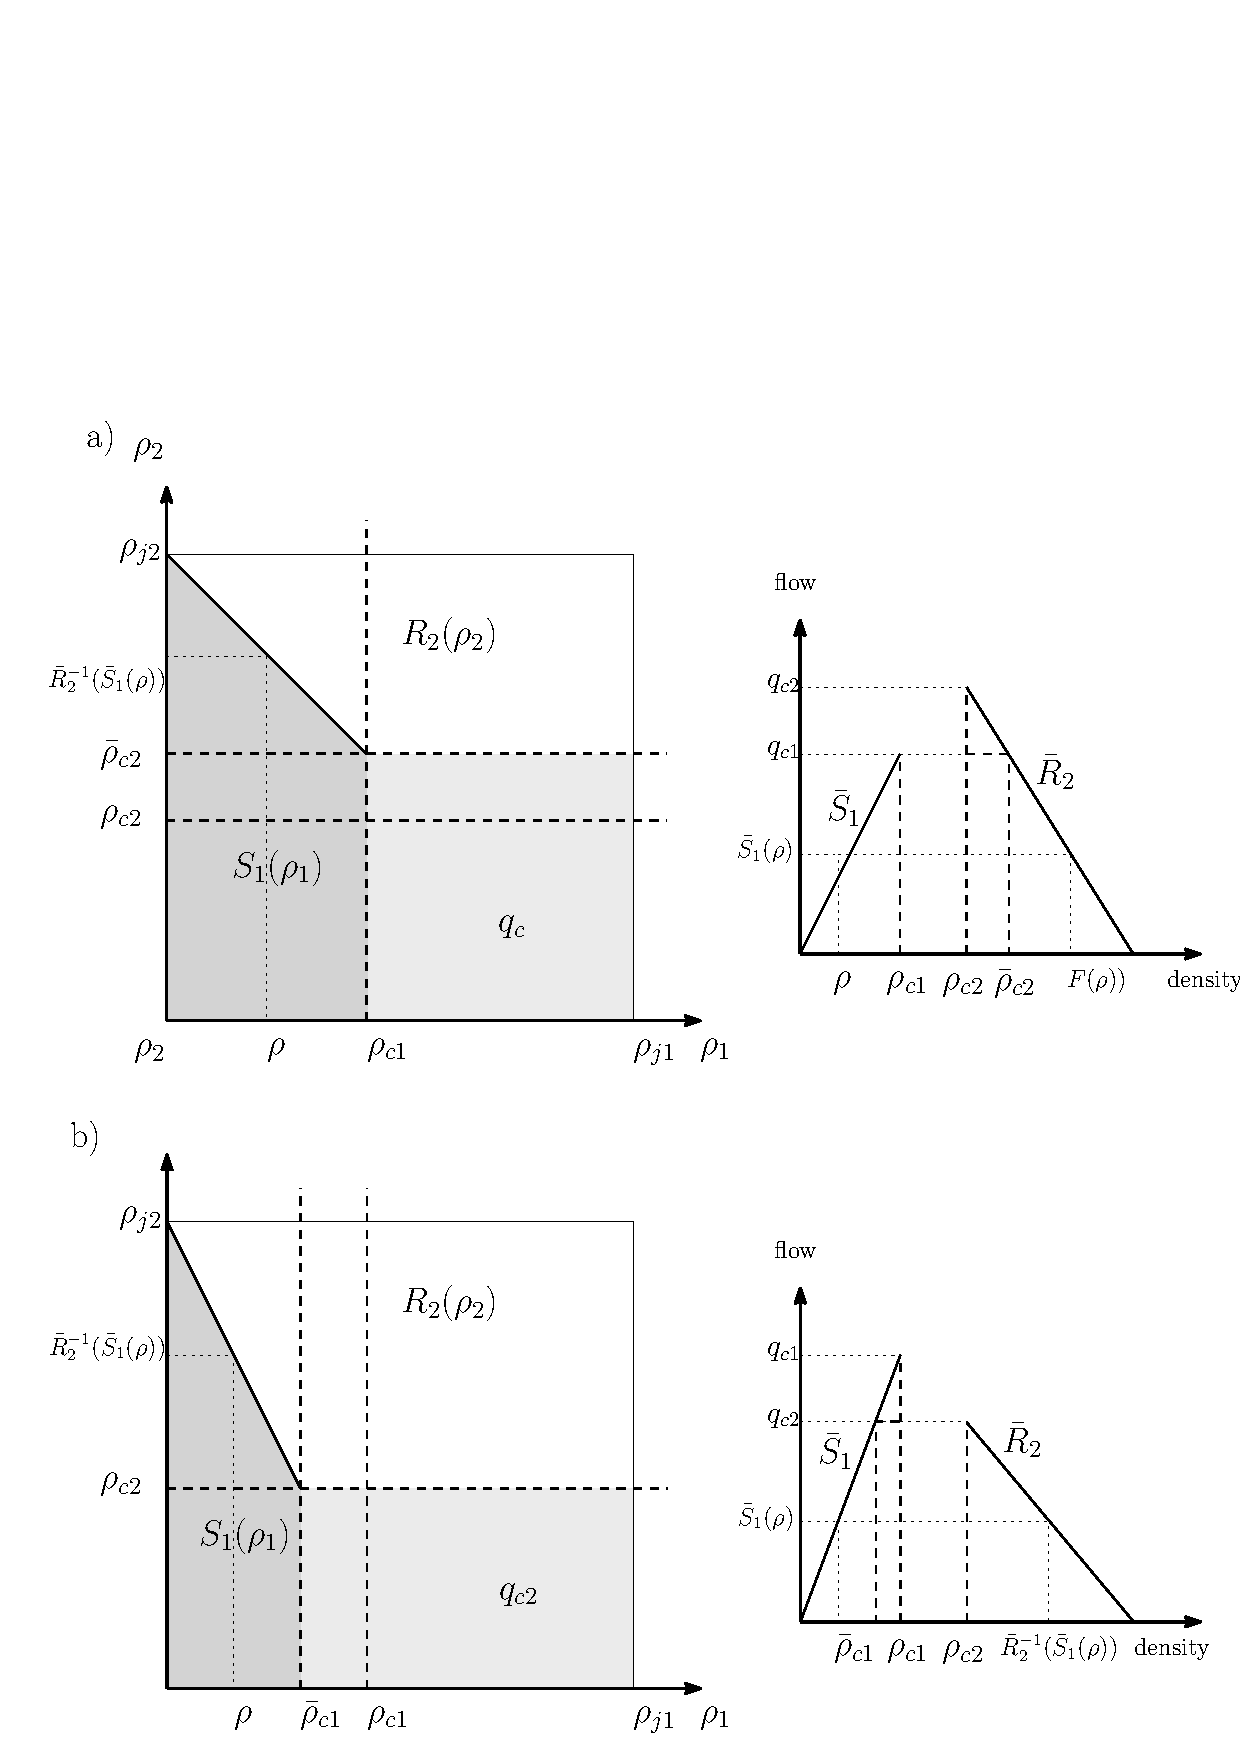
\includegraphics[width=12cm]{godunovDiagram3.pdf}
    \caption{Values of $G(\rho_{1},\rho_{2})$ in the space $(\rho_{1},\rho_{2})$ for the Daganzo-Newell fundamental diagram with different capacities $q_{c1} < q_{c2}$ for a) and $q_{c1} > q_{c2}$ for b). Note that for illustration purposes we suppose $\rho_{c1}\leq\rho_{c2}$.}
    \label{fig:godunovDiagram3}
\end{figure}

In this section, we study the CTM for a heterogeneous road, i.e. $\omega_{f}$, $v_{f}$, $\rho_{j}$, $\rho_{c}$, $q_{c}$ can vary along the link and we add the subscript $i$: $\alpha_{i}$, $\omega_{fi}$, $v_{fi}$, $\rho_{ji}$, $\rho_{ci}$, $q_{ci}$ for the parameters of the fundamental diagram $Q_{i}$ at cell $i$, and the associated sending and receiving flows $S_{i}$, $R_{i}$. Figure \ref{fig:godunovDiagram3} shows the explicit values taken by $G(\rho_{1},\rho_{2})$ in different regions of the space $(\rho_{1},\rho_{2})$ when $q_{c1} < q_{c2}$. We note that the critical density $\rho_{c2}$ is increased to the \textit{effective} critical value $\bar{\rho}_{c2}$ for the receiving flow $R_{2}$, with $\bar{\rho}_{c2} = \bar{R}^{-1}_{2}(q_{c1})$, and the \textit{effective} capacity is $\bar{q}_{c} = q_{c1}$, which is the capacity of the sending flow $S_{1}$. And Figure \ref{fig:godunovDiagram3} also shows the explicit values taken by $G(\rho_{1},\rho_{2})$ in different regions of the space $(\rho_{1},\rho_{2})$ when $q_{c1} > q_{c2}$. Similarly, the critical density $\rho_{c1}$ is decreased to the \textit{effective} value $\bar{\rho}_{c1}$ for the sending flow $S_{1}$ with $\bar{\rho}_{c1} = \bar{S}^{-1}_{1}(q_{c2})$, and the \textit{effective} capacity is $\bar{q}_{c} = q_{c2}$, which is the capacity of the receiving flow $R_{2}$. The Godunov flux has a more general expression \ref{eq:rhoGodunovFlux2}:

\begin{equation}
G(\rho_{1},\rho_{2}) = \begin{cases}
R_{2}(\rho_{2}) & \text{if } (\rho_{1},\rho_{2}) \in \textbf{W}\\
\bar{q}_{c} & \text{if } (\rho_{1},\rho_{2}) \in \textbf{L}\\
S_{1}(\rho_{1}) & \text{if } (\rho_{1},\rho_{2}) \in \textbf{D}
\end{cases}
\label{eq:rhoGodunovFlux2}
\end{equation}

\begin{equation}
\begin{array}{lll}
\textbf{W} & = \{(\rho_{1},\rho_{2}) \mid & \rho_{2} > F(\rho_{1}) \text{ ,   } \rho_{2} > \bar{\rho}_{c2}\}\\
\textbf{L} & = \{(\rho_{1},\rho_{2}) \mid & \rho_{1} > \bar{\rho}_{c1} \text{ ,   } \rho_{2} \leq \bar{\rho}_{c2}\}\\
\textbf{D} & = \{(\rho_{1},\rho_{2}) \mid & \rho_{2} \leq F(\rho_{1}) \text{ ,   } \rho_{1} \leq \bar{\rho}_{c1}\}
\end{array}
\label{eq:regionsHetero}
\end{equation}

\noindent where the boundary between the white and grey regions follows the $(\rho_{1},\rho_{2})=(\rho_{1},F(\rho_{1}))$ trajectory with $F(\rho_{1})= \bar{R}^{-1}_{2}(\bar{S}_{1}(\rho_{1}))$ for $\rho_{1} \leq \rho_{c1}$. $\bar{S}$ and $\bar{R}$ denote the restrictions of the sending and receiving flows to the sub-regions $[0,\rho_{c})$ and $(\rho_{c},\rho_{j}]$ respectively, which also correspond to the left and right parts (w.r.t. $\rho_{c}$) of the fundamental diagram, as shown in the Figure \ref{fig:godunovDiagram3}.

\noindent When the velocity is the Daganzo-Newell function (\ref{eq:dnVelocity}), the Godunov Flux \ref{eq:rhoGodunovFlux2} becomes \ref{eq:rhoGodunovFlux3}:

\begin{equation} \label{eq:rhoGodunovFlux3a}
G_{DN}(\rho_{1},\rho_{2}) = \begin{cases}
-\omega_{f2} \left( \rho_{2} - \rho_{j2} \right) & \text{if } (\rho_{1},\rho_{2}) \in \textbf{W}\\
\bar{q}_{c} & \text{if } (\rho_{1},\rho_{2}) \in \textbf{L}\\
v_{f1} \rho_{1} & \text{if } (\rho_{1},\rho_{2}) \in \textbf{D}
\end{cases}
\end{equation}

\noindent and the boundary between the white and dark-grey regions is:

\begin{equation} \label{eq:boundaryHetero}
(\rho_{1},\rho_{2})=(\rho_{1},-\frac{v_{f1}}{\omega_{f2}}\rho_{1}+\rho_{j2})
\end{equation}

\noindent And \textbf{W}, \textbf{L}, \textbf{D} form a polyhedral partition of the space:

\begin{equation}
\begin{array}{lll}
\textbf{W} & = \{(\rho_{1},\rho_{2}) \mid & \rho_{2} + \frac{v_{f1}}{\omega_{f2}}\rho_{1} > \rho_{j2} \text{ ,   } \rho_{2} > \bar{\rho}_{c2}\}\\
\textbf{L} & = \{(\rho_{1},\rho_{2}) \mid & \rho_{1} > \bar{\rho}_{c1} \text{ ,   } \rho_{2} \leq \bar{\rho}_{c2}\}\\
\textbf{D} & = \{(\rho_{1},\rho_{2}) \mid & \rho_{2} + \frac{v_{f1}}{\omega_{f2}}\rho_{1} \leq \rho_{j2} \text{ ,   } \rho_{1} \leq \bar{\rho}_{c1}\}
\end{array}
\label{eq:regions4}
\end{equation}

At cell $i$, this implies the effective density $\bar{\rho}^{u}_{ci}$ associated with the upstream boundary can be different from the effective density $\bar{\rho}^{d}_{ci}$ associated with the downstream boundary, depending of the capacity drops at these boundaries. Hence, using the notations introduced in section \ref{sec:decompositionModes} all the combinations between $(\rho_{-},\rho)$ and $(\rho,\rho_{+})$ can be possible so we have nine modes. Consequently, for a discretization in $n$ cells, the number of possible modes is $3^{n+1}$.

\begin{table}[ht]
\centering % used for centering table
\begin{tabular}{|c|c|c|c|c|c|}
  \hline
 number of cells & 1 & 2 & 5 & 10 & 20\\
  \hline
 number of modes & 9 & 27 & 729 & 177147 & $10^{10}$\\
  \hline
\end{tabular}
\label{table:numModes2} % is used to refer this table in the text
\caption{Number of modes for a heterogeneous road.}
\end{table}

\section{Kalman filtering-DRAFT}

and $F_{LH}[.]$, have the same expression with $f_{DN}(.)$ and $f_{LH}(.)$ respectively (as defined in Table. For instance, when we have a Daganzo-Newell fundamental diagram with update operator for the dynamic system $F_{DN}[.]$ (i.e. $\boldsymbol\rho^{t} = F_{DN}[\boldsymbol\rho^{t-1}]$), and suppose that the mode at $x=i$ is three ($m_{i}=3$) then\footnotemark: 

\begin{equation}
F_{i}[\boldsymbol\rho^{t-1}] = f_{DN,m_{i}}(\rho^{t-1}_{i_{-},i,i_{+}}) = f_{DN,3}(\rho^{t-1}_{i_{-},i,i_{+}}) = 
\rho^{t-1}_{i} + \alpha \omega_{f}\rho^{t-1}_{i+1} - \alpha \omega_{f}\rho_{c}
\label{eq:example}
\end{equation}

\footnotetext{
As we have seen earlier, $\alpha$, $\omega_{f}$, $v_{f}$, $\rho_{j}$, $\rho_{c}$, $q_{c}$ can vary along the link and a proper notation would be $\alpha_{i}$, $\omega_{fi}$, $v_{fi}$, $\rho_{ji}$, $\rho_{ci}$, $q_{ci}$ for the parameters of the fundamental diagram at $x=i$, so that:
\[
F_{i}[\rho^{t-1}] = f_{DN,m_{i}}(\rho^{t-1}_{i_{-},i,i_{+}}) = f_{DN,3}(\rho^{t-1}_{i_{-},i,i_{+}}) = 
\rho^{t-1}_{i} + \alpha_{i} \omega_{fi}\rho^{t-1}_{i+1} - \alpha_{i} \omega_{fi}\rho_{ci}
\]
}

In order to use the \textit{Extended Kalman filter} to estimate the state of the link given a sequence of noisy observations, we model the process in accordance with the framework of the \textit{Extended Kalman filter} by adding a white noise to the underlying dynamic system model. The ''true'' state $\boldsymbol\rho^{t}$ is then:

\begin{equation}
\boldsymbol\rho^{t} = F[\boldsymbol\rho^{t-1}] + \boldsymbol\eta^{t}
\label{eq:underlyingSystem3}
\end{equation}

\noindent where $\boldsymbol\eta^{t}\sim N(0,Q_{t})$ is the Gaussian zero-mean, white state noise with covariance $Q_{t}$. The estimated state at time $t$ is denoted by $\hat{\boldsymbol\rho}^{t}$ and the estimated covariance by $P_{t}$. The \textit{prediction step} gives the \textit{a priori} state estimate and covariance $\hat{\boldsymbol\rho}^{t:t-1}$ and $P_{t:t-1}$:

\begin{equation}
\begin{array}{ll}
\text{Predicted state estimate: } & \hat{\boldsymbol\rho}^{t:t-1} = F[\hat{\boldsymbol\rho}^{t-1}]\\
\text{Predicted covariance estimate: } & P_{t:t-1} = F_{t-1}P_{t-1}(F_{t-1})^{T} + Q_{t-1}
\end{array}
\end{equation}

\noindent where $F_{t}$ is the state transition defined to be the following Jacobian:

\begin{equation}
F_{t} = \left(\frac{\partial F_{i}[\rho^{t}]}{\partial \rho^{t}_{j}}\right)_{i,j}
\label{eq:jacobian2}
\end{equation}

The estimated mode $\hat{\boldsymbol m}^{t}$ associated to the estimated vector state $\hat{\rho}^{t}$ is defined from Table \ref{table:modes}. Specifically, in the context of our traffic model, the density at $x=i$ only depends on the densities at the neighbor points $x=i-1,i,i+1$. So $F_{t}$ is a $(n+2)\times(n+2)$ tridiagonal matrix, such that the diagonal elements are $\{0, J_{\hat{m}_{1},2},...,J_{\hat{m}_{n},2},0\}$, the lower diagonal elements are $\{J_{\hat{m}_{1},1},J_{\hat{m}_{2},1},...,J_{\hat{m}_{n},1},0\}$, and the upper diagonal elements are $\{0,J_{\hat{m}_{1},3},J_{\hat{m}_{2},3},...,J_{\hat{m}_{n},3}\}$, where $J$ is defined in Equation \ref{eq:jacobian}. 

In the case of the Daganzo-Newell fundamental diagram, the operator $F_{DN}[.]$ defined in (\ref{eq:underlyingSystem2}) is \textit{linear} (from the linearity of $f_{DN}$). Along with the assumption of a white state noise, the \textit{prediction step} (\ref{eq:predict}) of the \textit{Extended Kalman filter} is actually identical to the regular \textit{Kalman filter}, and it is known from the theory that the \textit{Kalman filter} is optimal \cite{Anderson2005}.

In the case of a linear-hyperbolic velocity function, the operator $F_{LH}[.]$ is not linear if at some points of the discrete space the mode is between four and seven. Then the \textit{Extended Kalman filter} is \textit{near-optimal}.

We can note that the first line and first column of $P_{t}$ have only zero elements because the boundary condition $\rho^{t}_{0}$ is deterministic (i.e. $cov(\rho^{t}_{0},\rho^{t}_{i})=0$ for $i=1,...,n$), and similarly the last line and last column of $P_{t}$ are null since the boundary condition $\rho^{t}_{n+1}$ is deteministic. Additionally, the observation model for the link is given by:

\begin{equation}
\boldsymbol y^{t} = H_{t}\boldsymbol\rho^{t} + \boldsymbol\chi^{t}
\end{equation}

\noindent where $H_{t}\in \{ 0,1 \}^{p_{t}\times n}$ is the linear observation observation matrix which encodes the $p_{t}$ observations (each one of them being at a discrete cell on the highway) for which the density is observed during discrete time step $t$, and $n$ is the number of cells along the link. The last term in (\ref{eq:observation}) is the white, zero mean observation noise $\boldsymbol\chi^{t} \sim N(0,R_{t})$ with covariance matrix $R_{t}$. The \textit{update step} is:

\begin{equation}
\begin{array}{ll}
\text{Kalman gain: } & K_{t} = P_{t:t-1}H_{t}^{T}\left(H_{t}P_{t:t-1}H_{t}^{T}+R_{t}\right)^{-1}\\
\text{Updated state estimate: } & \hat{\boldsymbol\rho}^{t} = \hat{\boldsymbol\rho}^{t:t-1} + K_{t}(\boldsymbol y^{t} - H_{t}\hat{\boldsymbol\rho}^{t:t-1})\\
\text{Updated estimate covariance: } & P_{t} = (I - K_{t}H_{t})P_{t:t-1}
\end{array}
\end{equation}

The Extended Kalman filter provides the distribution of $\hat{\boldsymbol\rho}^{t}$ given the sequence of observations $\boldsymbol y^{0:t}$, sequence of modes $\hat{\boldsymbol m}^{0:t} = \{\hat{\boldsymbol m}^{0},...,\hat{\boldsymbol m}^{t}\}$, and sequence of control parameters $\boldsymbol u^{0:t}$, which is exactly equal to the distribution of $\hat{\boldsymbol\rho}^{t}$ since the sequence $\hat{\boldsymbol m}^{0:t}$ is deterministic. Concretely, the vector of control parameters $\boldsymbol u^{t}$ contain the vector of critical densities $\boldsymbol\rho_{c}$, the vector of jam densities $\boldsymbol\rho_{j}$, and the boundary conditions $\rho^{t}_{0}$ and $\rho^{t}_{n+1}$. Theoretically, the result is obtained by marginalizing the joint distribution of $\hat{\boldsymbol\rho}^{t}$ and $\hat{\boldsymbol m}^{0:t}$ as follows:

\begin{equation}
\begin{array}{ll}
p(\hat{\boldsymbol\rho}^{t}|\boldsymbol y^{0:t},\boldsymbol u_{0:t}) & =
\int_{\mathcal{M}_{n}} p(\hat{\boldsymbol\rho}^{t}|\boldsymbol y^{0:t},\boldsymbol u^{0:t},\boldsymbol m^{0:t})p(\boldsymbol m^{0:t}|\boldsymbol y^{0:t},\boldsymbol u^{0:t})
d\boldsymbol m^{0:t}\\ 
& = \int_{\mathcal{M}_{n}} p(\hat{\boldsymbol\rho}^{t}|\boldsymbol y^{0:t},\boldsymbol u^{0:t},\boldsymbol m^{0:t})\boldsymbol 1_{\hat{\boldsymbol m}^{0:t}}d\boldsymbol m^{0:t}\\[1ex]
& = p(\hat{\boldsymbol\rho}^{t}|\boldsymbol y^{0:t},\boldsymbol u^{0:t},\hat{\boldsymbol m}^{0:t})
\label{eq:marginalization}
\end{array}
\end{equation}

\section{Implementation-DRAFT}

\subsection{Algorithm for the \textit{prediction step}}

Algorithm using the structure of $F_{t}$ and extension to a network

From Appendix \ref{sec:modes},  In (\ref{eq:predict}), the \textit{a priori} state estimate $\hat{\boldsymbol\rho}^{t:t-1}$ is derived through the algorithm in (\ref{eq:underlyingSystem2}).

\subsection{Accuracy}

For a Daganzo-Newell fundamental diagram, we can note that the decomposition in different modes in (\ref{eq:underlyingSystem2}) is in fact a special case of \textit{Conditional Dynamic Linear Model} (CDLM) as described in \cite{Chen2000} with a discrete latent indicator that is deterministic. In this case, there is only one estimated deterministic sequence of modes $\hat{\boldsymbol m}^{0:t}$ or latent indicators, hence there is no need to use a sequential Monte-Carlo method to sample an ensemble of trajectories of modes. The Mixture Kalman Filter \cite{Chen2000} reduces to a simple Kalman Filter. For non-triangular fundamental diagrams which have the characteristics \textbf{LWR1-6}, a first order Taylor Series expansion is applied. Such a linearization is a good approximation. Then the Extended Kalman filter can be applied to each mode.

In our case, the estimated sequence of modes $\hat{\boldsymbol m}^{0:t}$ is readily infered through the Godunov scheme, and at all the cells along the link, including those where there is no observation. Contrary to some previous models as in \cite{Munoz2003}, the modes are not directly sampled from density measurements along the highway. However, the mode is still indirectly infered from those measurements by assimilating the observations with the \textit{update state} of the Kalman filter. Besides, we rely on the accuracy of the estimation of the mode provided by the Godunov scheme when we apply the Kalman filter for each mode. Such an assumption that favors the mode provided by the Godunov scheme is yet another reason why the sequential Monte-Carlo method (with the resampling step) is not used in the algorithm, because we then suppose that our sequence of modes is the one with the largest likelihoods. (to develop, do a test of likelihood)

\subsection{Complexity}

Comparison with the Extended Kalman filter and matlab simulations and results

\bibliography{myBiblio}
\bibliographystyle{plain}

\end{document}
